\documentclass{fast-nuces-bs}
\usepackage{graphicx}
\usepackage{float}
\usepackage{blindtext}
\usepackage{mathptmx}% Times Roman font
\usepackage[T1]{fontenc}
\usepackage{lipsum} 
\usepackage{sectsty}
\usepackage{hyperref}
\usepackage{tikz-uml}
\usepackage{titlesec}
\titlespacing{\section}{0pt}{\parskip}{-\parskip}
\titlespacing{\subsection}{0pt}{\parskip}{-\parskip}

% Information about the Thesis 
% -----------------------------------------------------------------------------
% (All are compulsory, do not delete any line other than author Information)
% For e.g., usually there are 3 students in a group, so leave authorone, 
% authortwo, and authorthree, and delete authorfour.
%%%%%%%%%%%%%%%%%%%%%%%%%%%%%%%%%%%%%%%%%%%%%%%%%%%%%%%%%%%%%%%%%%%%%%%%%%%%%%%
\department{Department of Computer Science}
\faculty{Computer Science}
\degreeyear{2024}
\degreemonth{June}
\degreename{Bachelors in Computer Science}
\campuscity{Peshawar}
\authorone{Dawood Sarfraz}{20P-0153}
\authortwo{Waleed Akram}{20P-0640}
\authorthree{Shoaib Akhtar}{20P-0147}
\supervisor{Dr. Muhammad Amin}
\sessionduration{2020-2024}
\deanname{Dr. Dean Computing}
\directorname{Dr. Omar Usman Khan}
\hodname{Mr. Fazl-e-Basit}
\fypcoordinatorname{Mr. Haroon Zafar}
\title{MetaMed VR: Enhancing Medical Education through Immersive Virtual Reality}
%%%%%%%%%%%%%%%%%%%%%%%%%%%%%%%%%%%%%%%%%%%%%%%%%%%%%%%%%%%%%%%%%%%%%%%%%%%%%%%

%%%%%%%%%%%%%%%%%%%%%%%%%%%%%%%%%%%%%%%%%%%%%%%%%%%%%%%%%%%%%%%%%%%%%%%%%%%%%%
% Former document starts below this
\begin{document}
	
	\begin{acknowledgements}
		This project would not have been possible without the support of many dedicated individuals. Our deepest gratitude goes to our advisor, Dr. Muhammad Amin, for his invaluable feedback and unwavering guidance throughout the numerous revisions. We are also profoundly thankful to our coordinator, Mr. Haroon Zafar, for his continuous support and encouragement.
		
		We extend our sincere thanks to the entire Computer Science faculty for their mentorship and valuable time. Additionally, we are grateful to the National University of Computer and Emerging Sciences for providing the opportunity and financial support necessary to bring this project to fruition.
	\end{acknowledgements}
	\begin{abstract}
		The rapid evolution of technology continues to redefine traditional educational paradigms. This report delves into the pioneering exploration of leveraging Immersive Virtual Reality (VR) to transform medical education. Focused on the project \textbf{" Enhancing Medical Education through Immersive Virtual Reality (MetaMed) "} our study aims to revolutionize the pedagogical landscape of medical training.
		\\
		In the initial phase of our project, we embarked on a journey to harness cutting-edge VR technology. The objective was to create immersive learning environments that simulate real-world medical scenarios, allowing students to engage in interactive, hands-on learning experiences. Through the integration of advanced VR techniques, our project aspires to bridge the gap between theoretical knowledge and practical application, fostering a deeper understanding of medical concepts.
	\end{abstract}
	\chapter{Introduction}
\label{sec:introduction}
\begin{itemize}
\item Metaversion is a virtual universe that integrates VR, AR, and the Internet, providing a shared, immersive, and often three-dimensional space for online interaction and presence.
\item The Metaverse is a virtual world where users interact with digital avatars that reflect their identity and physical characteristics.
\item Metaversion, incorporating virtual offices, classrooms, and training environments, offers new opportunities for learning, skill development, and remote collaboration in both entertainment and education.
\end{itemize}
\section{History of the Metaverse}
Metaversion, also known as collective virtual shared space or virtual reality space, has a rich history rooted in science fiction, technology, and online communities. Here's a brief overview of the meta version's history:
\subsection{1970 - Sci-Fi Origins:}
Neal Stephenson's 1992 novel "Snow Crash" popularized the concept of metaversion, a virtual reality space where users interact as avatars, serving as a conceptual basis for later developments.
\subsection{Early Virtual Worlds:}
In the late 1970s and 1980s, MUDs and MOOs were online environments that enabled multiple users to interact in text-based virtual worlds, paving the way for modern online communities.
\subsection{1990 - Emergence of 3D Virtual Worlds:}
In the 1990s, 3D virtual worlds like Second Life emerged, enabling users to create avatars, socialize, and build virtual environments, paving the way for immersive metaverse experiences.
\subsection{2000 - Online Games and Social Media:}
Online interactions and communities are transforming MMOs like World of Warcraft and social media platforms like Facebook and Twitter, fostering connected digital spaces.
\subsection{2010 - VR and AR:}
Virtual and augmented reality technologies, like Oculus Rift and HTC Vive, are revolutionizing metaversion by providing immersive virtual spaces through smartphones and AR glasses.

\subsection{Current developments:}
As of September 2021, companies are developing meta-related technologies like virtual reality, augmented reality, blockchain, and decentralized platforms, using NFTs to represent digital assets within the metaverse.
\section{The Future of the Metaverse}
Metaversion, a future of immersive virtual and augmented reality experiences, blockchain-based asset ownership, and economic opportunities, is expected to revolutionize various sectors, redefining social dynamics, raising concerns about privacy, security, regulation, and environmental sustainability.
\begin{figure}[h]
    \centering
    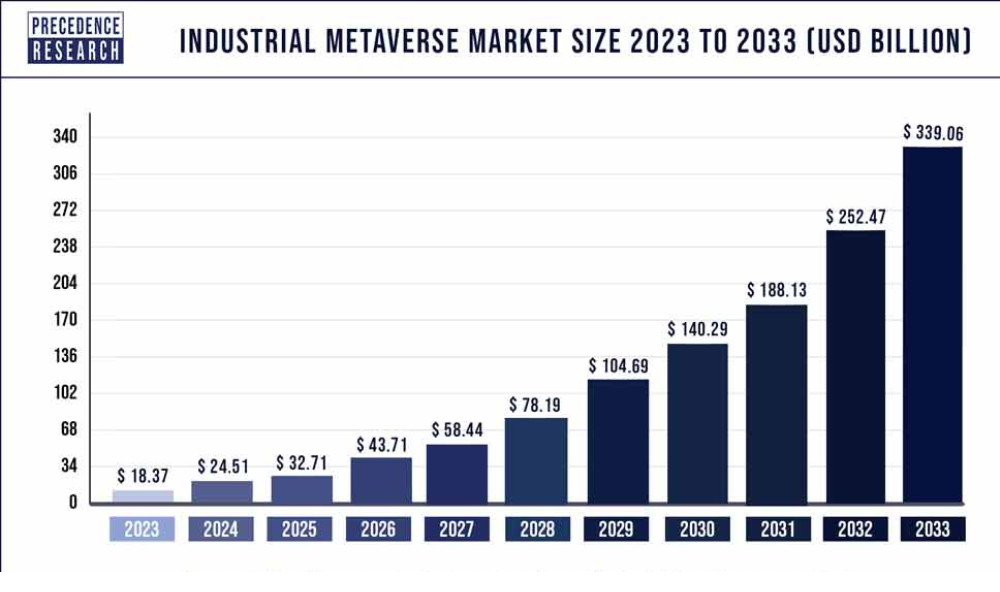
\includegraphics[width=0.8\textwidth, height=0.35\textheight]{Images/industrial-metaverse-market-size.png}
    \caption{Future of Metaverse}
    \label{fig:Future of Metaverse}\cite{metaverse-market}
\end{figure}
\section{How Metaverse Would Excel}
The success of the metaverse will be influenced by several key factors:\\
\textbf{Technology Advances:}\\ The metaverse's success relies on advancements in technologies like VR, AR, AI, and high-speed internet connectivity, along with enhanced hardware and software for immersive virtual experiences.\\
\textbf{User Adoption:}\\ The metaverse's success relies on a critical mass of active users, with user-friendly interfaces and accessibility playing a crucial role in attracting a diverse user base.\\
\textbf{Content and Creativity:}\\ The Metaverse requires a diverse range of engaging content, experiences, and activities, including virtual worlds, games, social spaces, art, and educational content, for easy creation and sharing.\\
\textbf{Interoperability and standards:}\\ Open standards and protocols for the metaverse are crucial for creating a seamless, accessible environment by facilitating interoperability between virtual worlds and platforms.\\
\textbf{Security and Privacy:}\\ Users must rely on metaverse for their personal data and transactions, requiring robust security measures, data protection, and privacy controls to prevent abuse, fraud, and unauthorized access.\\
\textbf{Economic Viability:}\\ Metaversion necessitates a sustainable economy, attracting users and content creators through virtual real estate, digital currencies, and employment opportunities, utilizing blockchain technology and NFTs.\\
\textbf{Regulation and governance:}\\ Governments and regulators will need to create clear guidelines and legal frameworks for meta
	\chapter{Literature overview}
\label{ch:lit-review}
This literature review explores the integration of metaversion in healthcare, highlighting its potential for innovative solutions such as medical training, telemedicine, mental health therapy, and patient empowerment. It examines historical perspectives, technological foundations, practical applications, ethical considerations, and future prospects.
\section{All one needs to know about metaverse: A complete survey on technological singularity, virtual ecosystem, and research agenda 
	\cite{lee2021all}\cite{BookChapter1}}
\textbf{Methodology:}\\The article explores the metaverse's evolution, highlighting core technologies like augmented reality, AI, and blockchain, user-centric factors like avatars, content creation, and virtual economies, and proposes a research agenda. \\
\textbf{Limitations:}\\The article offers a broad overview of metaverse evolution, but lacks in-depth analysis, discusses challenges like ethical issues and inequality, and relies on a survey-based approach without empirical support. \\
\textbf{Results:}\\Comprehensive framework for examining metaverse development.
Concrete research agenda for metaverse development
\section{Healthcare in metaverse: A survey on current metaverse applications in healthcare
	\cite{bansal2022healthcare}\cite{JournalArticle12}}
\textbf{Methodology:}\\
The article explores metaverse applications in healthcare, highlighting recent technological advancements, challenges, and potential improvements, emphasizing the need for sustainable, innovative solutions..\\
\textbf{Limitations:}\\Existing healthcare systems limitations revealed during COVID-19 pandemic. Surge in healthcare innovation using virtual environments for alternative systems. \\
\textbf{Results:}\\The metaverse for healthcare requires addressing connectivity, privacy, security, integration, interoperability, user experience, and technical issues with VR and AR technologies.
\section{Medical Metaverse: Technology, Applications, Challenges and Future
	\cite{shao2023medical}}
\textbf{Methodology}\\The paper explores the use of metaverse technologies in healthcare, identifying challenges and proposing solutions for efficient diagnosis, education, and treatment in healthcare settings.\\
\textbf{Limitations:}\\The paper provides a thorough overview of the Metaverse's potential in healthcare, highlighting its applications, technologies, and challenges, but lacks case studies and real-world implementations due to limited literature.\\
\textbf{Results:}\\ Review of technologies and applications of the metaverse. 
Exploration of potential and future direction in healthcare.
\section{The Metaverse for Healthcare: A Survey of Potential Applications, Challenges, and Future Directions.
	\cite{yendurimetaverse}\cite{JournalArticle10}}
\textbf{Methodology:}\\The paper explores the use of the Metaverse in healthcare, highlighting applications, technologies, and projects, while identifying challenges and proposing future research directions, focusing on AI, VR, AR, IoMT, robotics, and quantum computing.\\
\textbf{Limitations:}\\Adopting AI-enabled Metaverse in healthcare faces challenges like high-speed communication, massive computation, security concerns, data loss, heterogeneity of devices, and cost implications, impacting its comprehensiveness.\\
\textbf{Results:}\\
Medical education uses VR for learning body structures, improving future doctors' quality. However, AI-enabled Metaverse risks patient privacy and ethical issues, potentially leading to medical errors. Edge computing for real-time data retrieval requires additional devices, posing network scalability challenges.
\section{Revolutionizing Medical Education with Metaverse
	\cite{baskar2022revolutionizing}\cite{JournalArticle9}}
\textbf{Methodology:}\\Interdependence of characteristics in virtual teaching model.
Overcoming obstacles through technological advancements in education.\\
\textbf{Limitations:}\\The paper neglects to address technical challenges, adoption barriers, ethical considerations, and perspectives of educators, healthcare providers, and patients in integrating metaverse technology in medical education, including cost and infrastructure.\\
\textbf{Results:}\\ The paper focuses on methods for revolutionizing medical education using metaverse. It discusses the potential of metaverse in providing interactive and immersive experiences in healthcare.
\section{The Metaverse in Medical Education and Clinical Practice
	\cite{juan2023metaverse}}
\textbf{Methodology:}\\Use of immersive virtual and augmented environments.
Utilization of different models of stereoscopic vision glasses\\
\textbf{Limitations:}\\No specific limitations mentioned in the abstract. Further details on limitations not provided in the text.\\
\textbf{Results:}\\The paper presents immersive virtual and augmented environments for medical training. These environments use stereoscopic vision glasses to create a metaverse for enhanced medical training.
\section{Virtual reality and the transformation of medical education
	\cite{pottle2019virtual}}
\textbf{Methodology:}\\The paper discusses the use of simulation in clinical training but highlights its resource-intensive nature. It advocates for the adoption of virtual reality (VR) in medical education, highlighting its effectiveness in healthcare and its potential for providing quality, geographically independent training.\\
\textbf{Limitations:}\\
The paper generalizes VR's effectiveness in medical education without addressing specific limitations or challenges, lacks in-depth analysis of barriers, and overlooks technological constraints crucial for real-world implementation, presenting a one-sided view and overlooking areas for further research.\\
\textbf{Results:}\\Digital transformation has a great impact on medical education.
Inclusion of AI and VR benefits medical students.
\section{A Virtual Reality for the Digital Surgeon
	\cite{velazquez2021virtual}}
\textbf{Methodology:}\\The paper reviews VR technology's potential in healthcare, surgical education, and support tools, highlighting its potential to optimize patient data, improve surgical outcomes, and revolutionize healthcare.\\
\textbf{Limitations:}\\The paper's limited scope may limit its generalizability, overlooking challenges in implementing VR in healthcare. Additionally, reliance on a limited dataset or specific sources could affect the depth and reliability of the findings, potentially affecting the robustness of conclusions about VR's impact on surgical education and clinical practice.\\
\textbf{Results:}\\ VR has the potential to improve surgical education and skills.
VR can optimize preoperative planning and intraoperative support in clinical practice.
\section{Transforming medical education and training with VR using M.A.G.E.S.
	\cite{ProceedingsArticle}}
\textbf{Methodology:}\\The paper introduces a new VR software system for healthcare training, specifically Psychomotor Virtual Reality Surgical Training, which enhances surgeon skills through gamification and advanced interactability, and supports multiple surgeons and assistants.\\
\textbf{Limitations:}\\The paper primarily discusses orthopedic surgeries, neglecting generalizability, cost-effectiveness, VR surgical training solution validation, integrated educational curriculum effectiveness, long-term skill retention, and user experience feedback.\\
\textbf{Results:}\\The paper focuses on methods for revolutionizing medical education using metaverse. It discusses the potential of metaverse in providing interactive and immersive experiences in healthcare.
\section{Virtual Reality in Medicine
	\cite{JournalArticle}\cite{JournalArticle11}}
\textbf{Methodology}\\Multimodal interactions between user and virtual environment.
Technical requirements and design principles of input devices, displays, and rendering techniques.\\
\textbf{Limitations:}\\Physiological constraints. Technical requirements and design principles of multimodal input devices, displays, and rendering techniques.\\
\textbf{Results:}\\ Examples of virtual reality applications in surgical training, intra-operative augmentation, and rehabilitation. Provides technical requirements and design principles for virtual reality in medicine.
\section{A Virtual Environment for Training and Assessment of Surgical Teams
	\cite{papagiannakis2018virtual}}
\textbf{Methodology:}\\The paper explores the use of Collaborative Virtual Environments (CVEs) in surgical team training and assessment to enhance remote interactions and improve teamwork skills. The proposed CVE architecture supports team training and assessment in surgical simulations, reducing costs and requiring live subjects.\\
\textbf{Limitations:}\\Cost reduction for training is a limitation.
Use of guinea pigs and anatomical specimens is reduced.\\
\textbf{Results:}\\Proposed architecture for training and assessing team skills during surgery. Use of statistical models to monitor and assess team performance.
\section{Virtual reality technology and its application in modern medicine
	\cite{JournalArticle}}
\textbf{Methodology:}\\The paper discusses the use of virtual reality (VR) technology in medical applications such as surgery, telemedicine, and patient education, comparing it to traditional methods and highlighting its advantages and limitations.\\
\textbf{Limitations:}\\Limited access to VR technology in medical settings. Challenges in integrating VR into existing medical practices.\\
\textbf{Results:}\\ VR applied in virtual human, assisted diagnosis, surgery simulation. VR used in virtual telemedicine for medical purposes.
\section{Role of virtual reality for healthcare education
	\cite{BookChapter}}
\textbf{Methodology:}\\The research paper explores the use of VR technology in healthcare education, highlighting its role in storing patient data as 3D points, enhancing clinical skills, and providing flexible training for practitioners, ultimately improving the quality and standards of medical education.\\
\textbf{Limitations:}\\
Few are using VR to evaluate medical students' success. VR technology not widely used for medical training evaluation.\\
\textbf{Results:}\\ VR improves learning and training of medical practitioners.
VR enhances comprehension of anatomy and clinical outcomes.
\section{Next-Gen Mulsemedia: Virtual Reality Haptic Simulator’s Impact on Medical Practitioner for Higher Education Institutions
	\cite{journalarticle4}\cite{JournalArticle5}\cite{JournalArticle8}}
\textbf{Methodology:}\\ The study used the core motivation hypothesis to boost motivation in the classroom. The study used the attention, relevance, confidence, and satisfaction (ARCS) model to analyze the impact of virtual reality on student motivation and content update implementation.\\
\textbf{Limitations:}\\ Lack of research on consequences of virtual reality
Early stage of virtual reality technology research.\\
\textbf{Results:}\\ Virtual reality simulators improve student motivation and learning. VR has the potential to transform medical education.

\section{Design and implementation of a 3D digestive teaching system based on virtual reality technology in modern medical education
	\cite{Journal1}}
\textbf{Methodology:}\\
DX technologies: VR, AR, MR, XR, 3D images, holograms, AI. Utilization of HMDs, wearable sensors, 5G, and Wi-Fi.\\
\textbf{Limitations:}\\ Lack of systematic methodology, affecting evidence level
Heterogeneity in XR techniques studies, limiting systematic reviews.\\
\textbf{Results:}\\ The 3D digestive teaching system using VR significantly improved student understanding and retention, leading to higher test scores and increased engagement. This demonstrates VR's effectiveness in enhancing medical education.

\section{A Virtual Operating Room for Context-Relevant Training
	\cite{JournalArticle2}}
\textbf{Methodology:}\\
Virtual agents with unique personalities and knowledge structures defined. Immersive Virtual Operating Room (VOR) simulating surgical procedures described \\
\textbf{Limitation:}\\
Current medical simulators lack addressing errors in healthcare system. Existing simulators focus on procedural skills, not team dynamics.\\
\textbf{Results:}\\ Pilot session with surgical resident unfamiliar with VOR showed challenges. VOR allows team-based surgical training with virtual expert agents.

\section{Virtual reality surgical training and assessment system
	\cite{JournalArticle3}\cite{JournalArticle7}}
\textbf{Methodology:}\\ Soft-tissue model based on volumetric mass-spring system
Texture mapping for realistic organ representation and space perception.\\
\textbf{Limitation:}\\ Limits of realism in surgical simulation Challenges in obtaining reliable measures of surgical skills.\\
\textbf{Results:}\\ VR surgical system based on C-source code and OpenGL.
System handles accurate interactions between soft-tissue and surgical instruments
	\chapter{Project Vision}
\label{ch:vision}
\section{Problem Statement}
The project aims to provide medical students with hands-on experience through a virtual medical training platform, leveraging the metaverse to provide realistic scenarios and risk-free practice opportunities, overcoming challenges like limited availability and high costs.

\section{Goals}
The project aims to create a metaverse-based medical training platform, offering a risk-free environment for medical students to practice skills, enhance learning, and reduce costs and ethical concerns.

\section{Project Scope}
The project aims to create a metaverse-based medical training environment, incorporating realistic simulations, haptic feedback devices, and hands-on practice for various medical specialties.
\section{Limitations}
The project faces constraints such as budget constraints, metaverse platform technology limitations, ethical standards, time constraints, and regulatory compliance.

\section{Stakeholders}
Key stakeholders in this project include medical students, physician educators, healthcare institutions, and potentially patients who may benefit from better trained medical professionals.

	\chapter{Software Requirements Specification}
\label{ch:srs}
This chapter will contain the functional and non-functional requirements of the project.
\section{List of functions}
List of key features for the "Improving Medical Education through Immersive Virtual Reality (MetaMed)" project:\\
\textbf{Realistic medical simulations:}\\ Create highly realistic medical scenarios and procedures that faithfully mimic real medical experiences, including various medical specialties.\\
\textbf{Haptic feedback integration:}\\ Integrate tactile feedback devices to provide tactile sensations, increasing the realism of medical training and allowing students to develop their tactile skills.\\
\textbf{Immersive 3D Environments:}\\ Create immersive, 3D virtual environments that accurately represent medical settings, including operating rooms, medical instruments, and anatomical structures.\\
\textbf{Interactivity:}\\Enables hands-on interaction with virtual medical tools, instruments, and equipment, allowing students to perform medical tasks and procedures.\\
\textbf{Remote Access:}\\ Enable medical students to access a metaverse-based medical training platform from remote locations, facilitating flexible learning.
\section{Test plan (test level, test techniques)}
\text{Test plan for our project will be as:}
\begin{itemize}
    \item Movement in VR 
    \item Interaction with Objects
    \item Treatement to Patient
\end{itemize}
\section{Use Case Diagram}
Here is the Use Case Diagram of the Project.
\begin{figure}[h]
    \centering
    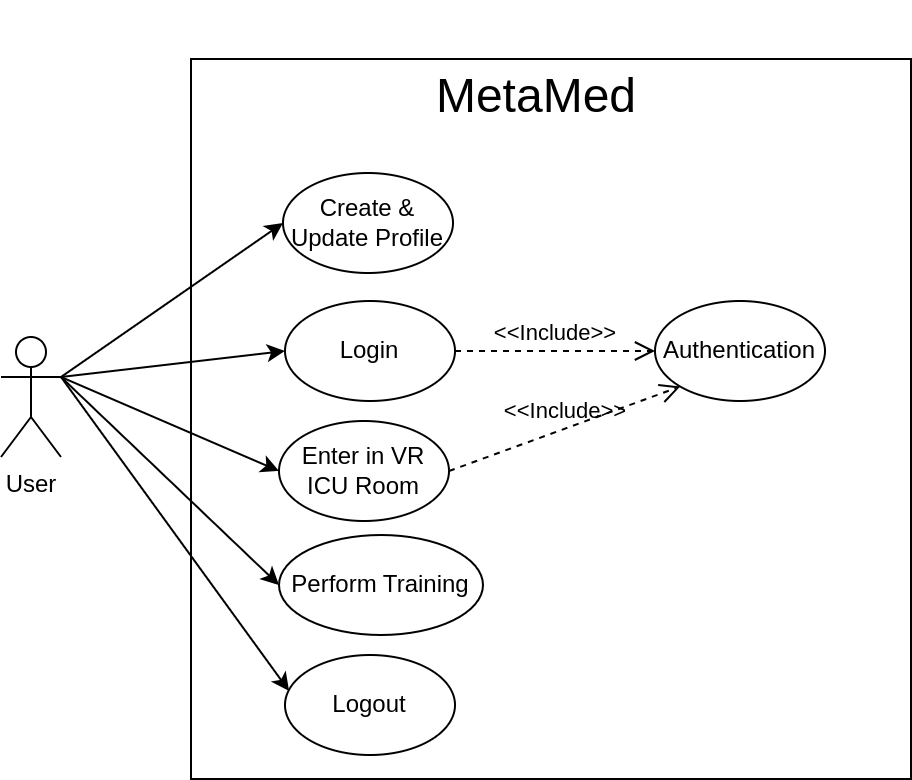
\includegraphics[width=0.6\textwidth, height=0.3\textheight]{Images/Use Case.drawio.png}
    \caption{Use Case Diagram}
    \label{fig:system-diagram}
\end{figure}

\section{Software Development Plan}
\text{Software Development Plan for our project will be as:}
\begin{itemize}
    \item Project Overview 
    \item Requirements Gathering and Analysis
    \item System Design
    \item Development
    \item Testing
    \item Documentation
    \item Management
\end{itemize}

\section{System Diagram}
It is the System Diagram of the Project.
\begin{figure}[h]
    \centering
    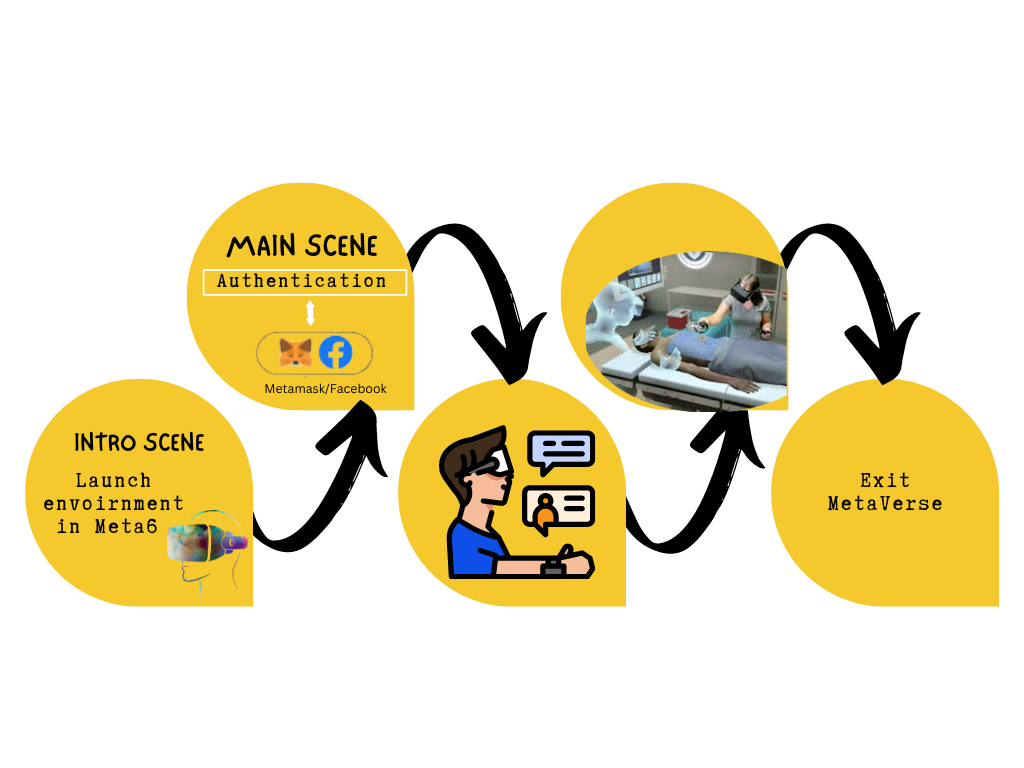
\includegraphics[width=1\linewidth, height=0.65\linewidth]{Images/system.png}
    \caption{System Diagram}
\end{figure}
\newpage
\section{Activity Daigram}
The activity diagram aims to illustrate the entire process of project working and demonstration.
\begin{figure}[h]
    \centering
    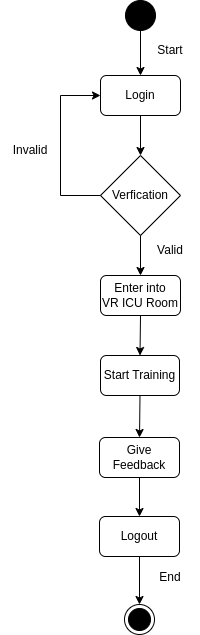
\includegraphics[width=0.25\linewidth]{Images/Activity.drawio.png}
    \caption{Activity Diagram}
\end{figure}
\newpage
\section{Tools and Technologies used}
These are some tools and technologies used in this project.
\subsection{C-Sharp:}
C-sharp is a programming language developed by Microsoft for use with the .NET Framework. It is widely used for developing web applications, desktop applications, mobile apps, games, and more. Known for its versatility and ease of use, C-sharp is popular in various software development fields. It supports object-oriented programming and provides a rich set of libraries, making it a powerful tool for developers.
%\begin{figure}[h]
%	\centering
%	
\includegraphics[width=0.1\linewidth, height=0.1\linewidth]{Images/CSharp.png}
%	\caption{C-Sharp\cite{csharp}}
%\end{figure}
\subsection{Blender}
Blender is a free, open-source 3D graphics software used for creating a wide range of visual content, including animated films, visual effects, art, and models. It also supports motion graphics, interactive applications, and virtual reality. Blender's versatility makes it popular among artists, animators, and developers. Its open-source nature allows for community-driven improvements and extensive customization. Blender is a powerful tool in the 3D graphics industry.
%\begin{figure}[h]
%	\centering
%	
\includegraphics[width=0.2\linewidth, height=0.2\linewidth]{Images/blender.png}
%	\caption{blender\cite{blender}}
%\end{figure}
\subsection{Git}
Git is a distributed version control system that tracks versions of files. It is used to control source code and collaboratively developing software. Git is a distributed version control system that efficiently manages and tracks changes in projects of any size. Created by Linus Torvalds in 2005, Git allows every developer to have a full copy of the project’s history, making it resilient and suitable for offline work.
%\begin{figure}[h]
%	\centering
%	
\includegraphics[width=0.15\linewidth, height=0.15\linewidth]{Images/git.png}
%	\caption{git\cite{git-logo}}
%\end{figure}
\newpage
\subsection{GitHub}
GitHub is a platform for developers to create, store, manage, and share their code, utilizing Git for distributed version control. It offers features like access control, task management, and continuous integration, making it a central hub for collaborative software development. GitHub facilitates project collaboration, allowing multiple contributors to work on the same codebase seamlessly. Its integration with Git ensures that changes are tracked, and the development process is efficient and organized.
%\begin{figure}[h]
%	\centering
%	
\includegraphics[width=0.1\linewidth, height=0.1\linewidth]{Images/GitHub.png}
%	\caption{GitHub\cite{github-logo}}
%\end{figure}
\subsection{Meta}
The Metaverse is a sophisticated, interconnected virtual world that enhances user experiences by offering seamless, immersive digital environments. It merges physical and virtual realities, allowing users to interact, work, and play within a shared, persistent digital space. This virtual universe encompasses everything from social interactions to business activities, powered by technologies like virtual reality (VR), augmented reality (AR), and blockchain. As the Metaverse evolves, it is expected to transform how we engage with digital content and each other, creating new opportunities for innovation and connection.
%\begin{figure}[h]
%	\centering
%	
\includegraphics[width=0.2\linewidth, height=0.2\linewidth]{Images/meta.png}
%	\caption{Meta\cite{meta}}
%\end{figure}
\subsection{Unity}
Unity is a versatile engine used for developing both 3D and 2D games, as well as interactive simulations. Its flexibility and user-friendly interface have led to widespread adoption across various industries beyond video gaming, including film, automotive, architecture, and education. Unity supports a range of platforms, enabling developers to create cross-platform applications with ease. Its robust asset store and strong community support make it a popular choice for creating immersive and engaging digital experiences.
%\begin{figure}[h]
%	\centering
%	
\includegraphics[width=0.2\linewidth,height=0.2\linewidth]{Images/unity.png}
%	\caption{Unity\cite{Unity}}
%\end{figure}
\newpage
\subsection{Meta Quest 2}
Project MetaMed VR used the Meta Quest 2 to leverage its advanced features such as hand tracking and gesture recognition, significantly enhancing medical education through immersive virtual reality experiences. The Meta Quest 2's capabilities provide a more interactive and engaging learning environment, allowing users to practice and visualize complex medical procedures in a virtual space. This innovative approach helps bridge the gap between theoretical knowledge and practical application, making medical training more effective and accessible.
%\begin{figure}[h]
%	\centering
%	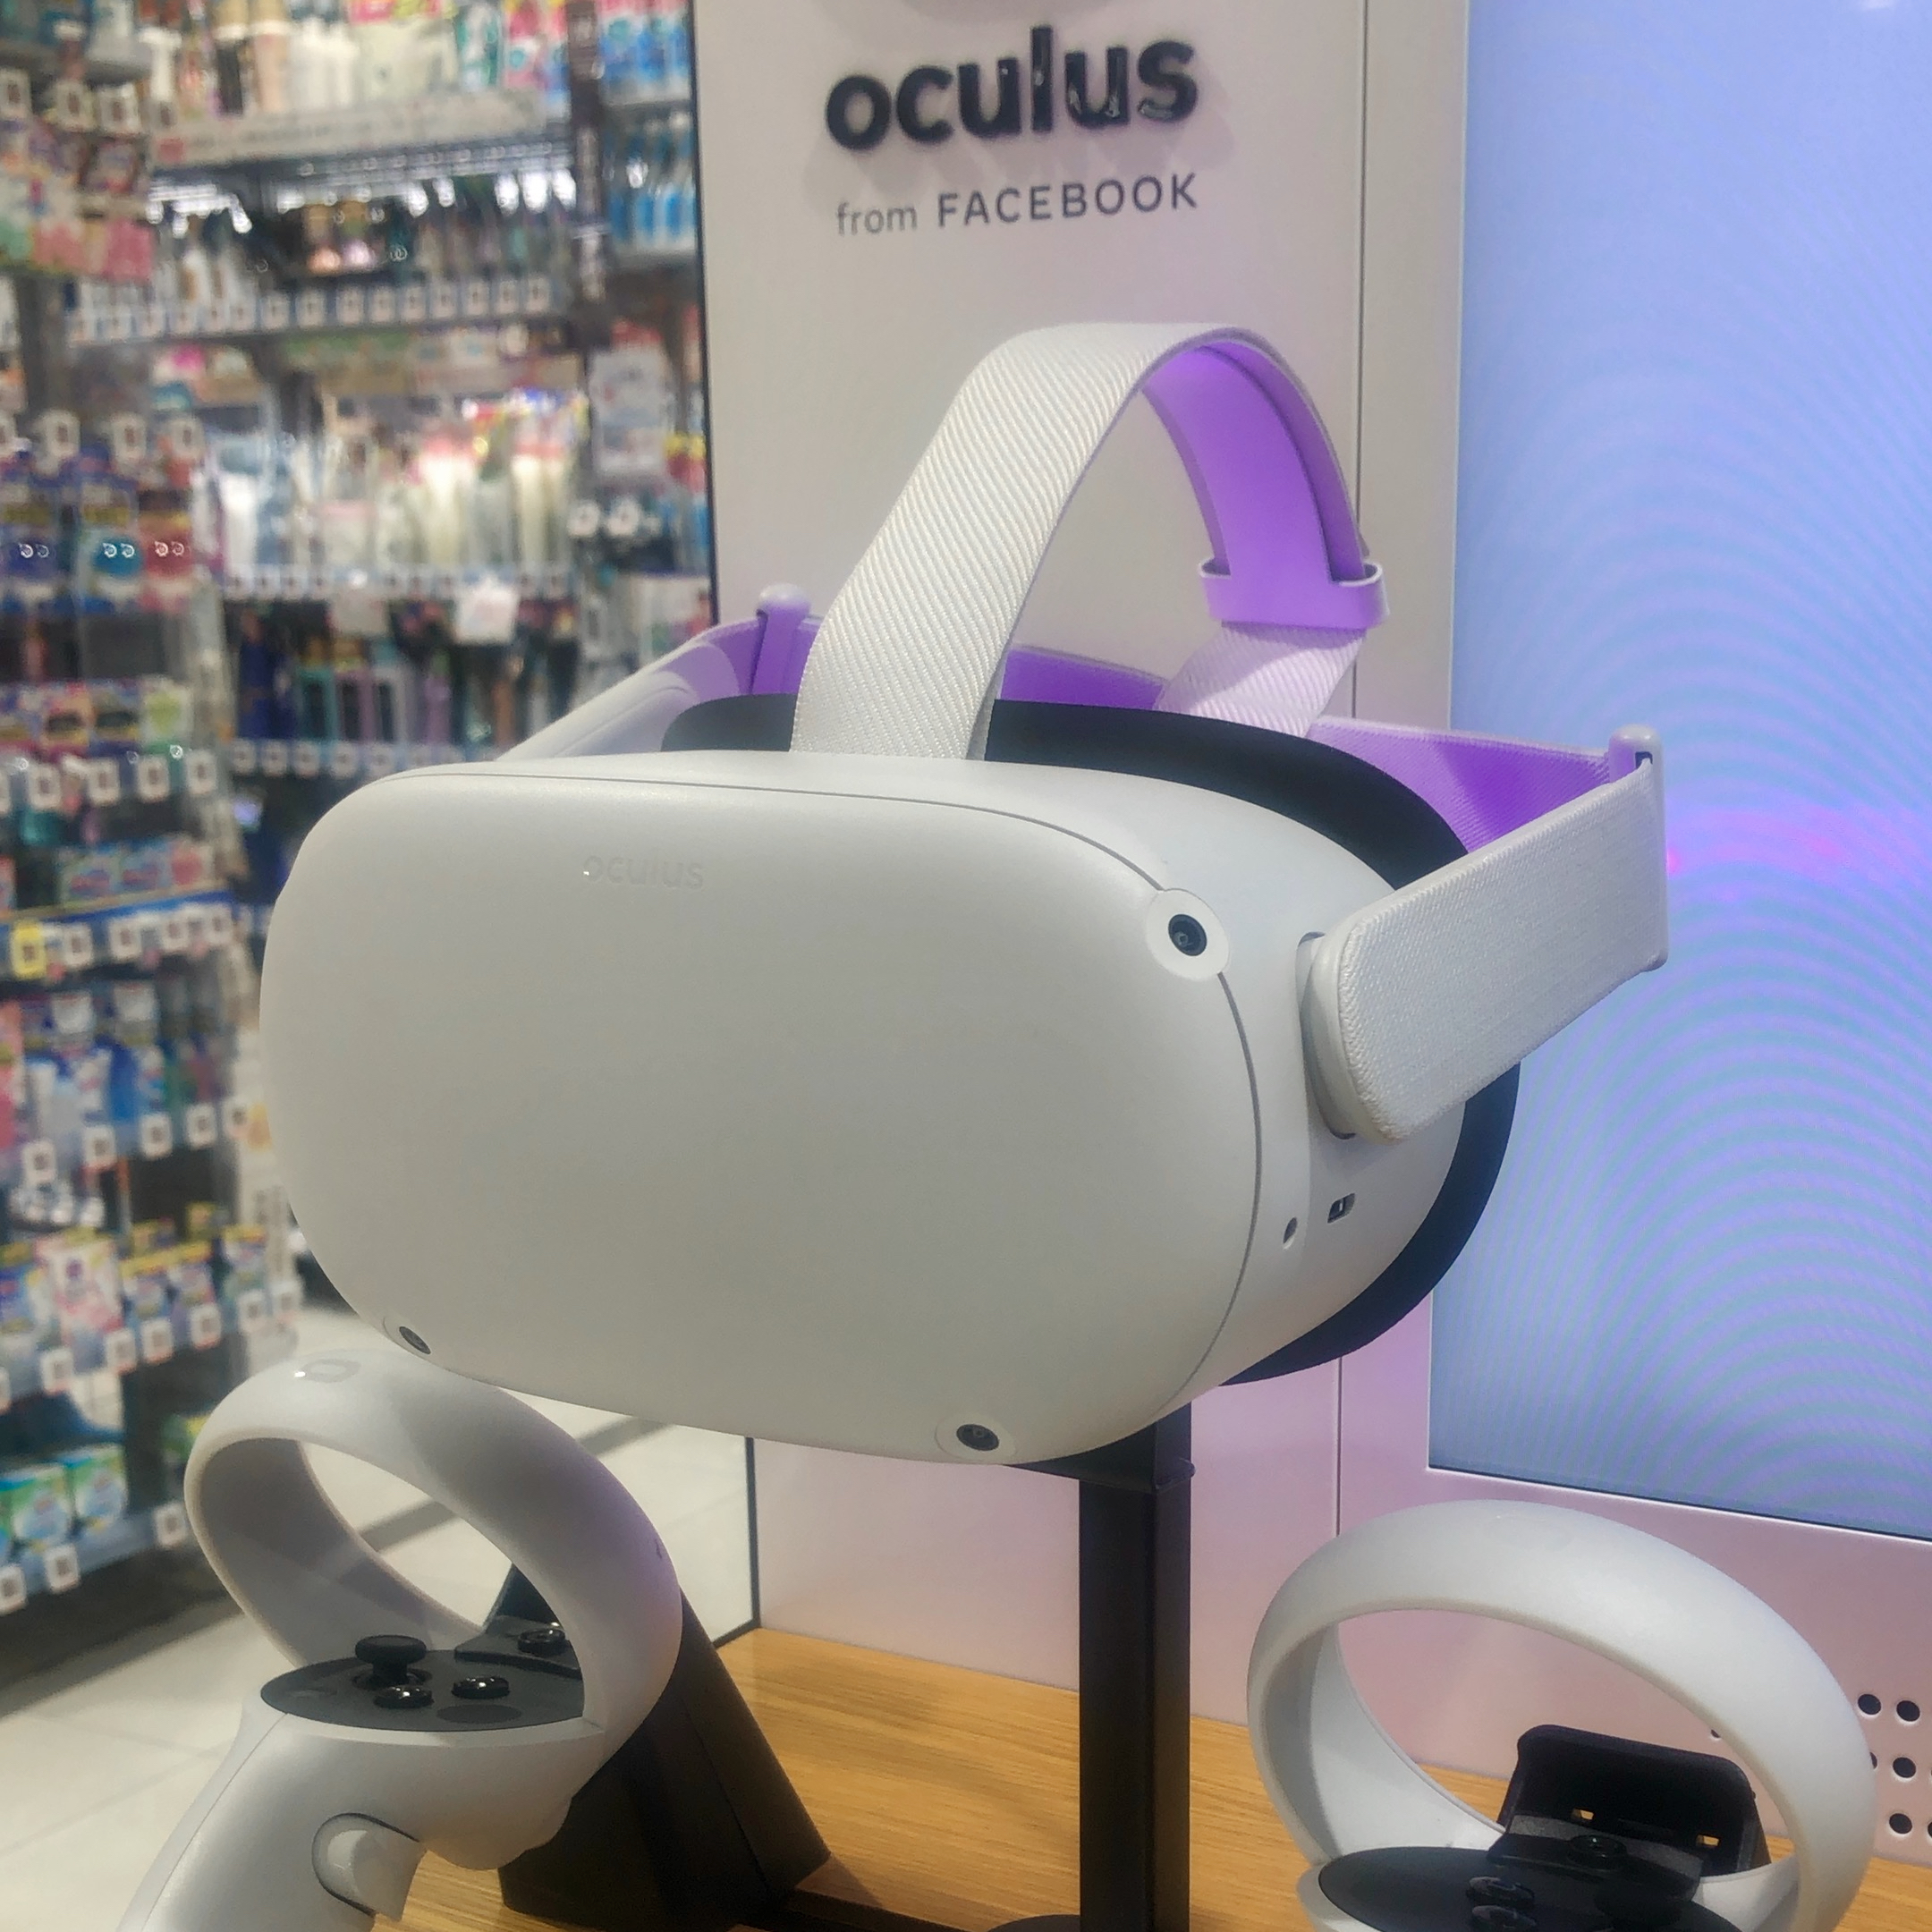
\includegraphics[width=0.4\linewidth,height=0.3\linewidth]{Images/metaquest2.png}
%	\caption{Meta Quest 2\cite{metaquest}}
%\end{figure}
\subsection{Microsoft Visual C++}
Microsoft Visual C++ is integrated with Unity 3D to optimize code, enhance performance, and manage memory in complex applications. This integration ensures smooth and efficient gameplay by providing advanced debugging, profiling, and optimization tools. Visual C++ helps developers address performance bottlenecks and memory management issues, which is crucial for creating high-quality, resource-intensive games and applications. By leveraging these capabilities, Unity developers can achieve better overall performance and stability in their projects.
%\begin{figure}[h]
%	\centering
%	
\includegraphics[width=0.2\linewidth,height=0.2\linewidth]{Images/VS Code.png}
%	\caption{Microsoft Visual C++\cite{visual-studio-icon}}
%\end{figure}
	\chapter{Iteration Plan}
\label{ch:iter0}
\section{Planning Strategy}
\text{Planning Strategy for our project will be as:}

\subsection{FYP 1 Mid:}
 
\begin{itemize}
	\item Literature review related Metaverse, and Healthcare
	\item Designed Use-case, System Diagram
\end{itemize}

\subsection{FYP 1 Final:}
\begin{itemize}
	\item Environment setup in Unity3D and Blender 
	\item Designed basic environment of Hospital like Rooms and Cadavers
	\item Delivered Demo of our environment
	
\end{itemize}


\subsection{FYP 2 Mid:}
\begin{itemize}
	\item User Movements
	\item Patient Information
	\item Medicines Information
	\item Basic Tools like syrings
\end{itemize}

\subsection{FYP 2 Final:}
\begin{itemize}
	\item Debugging
	\item Oculus Integration 
	\item Oculus Testing
\end{itemize}

	\chapter{Iteration 1 (FYP-1 Mid)}
\label{ch:iter1}
\begin{itemize}
    \item FYP 1 Mid: 
    \begin{itemize}
    \item Literature review related Metaverse, and Healthcare
    \item Designed Use-case, System Diagram
    \end{itemize}
\end{itemize}


\section{Literature review related Metaverse, and Healthcare}
{This literature review explores the potential of metaversion in healthcare, a virtual, interconnected digital realm. It examines current research, technology, and developments in metaversion, focusing on historical perspectives, technological foundations, practical applications, ethical considerations, and future prospects. The review aims to illuminate the current state of knowledge and pave the way for further advancements in this rapidly evolving field.
}

\section{Designed Use-case, System Diagram}
\begin{itemize}
    \item Use Case 
    \item System Diagram
    \item Activity Diagram
\end{itemize}


\section{Use Case Diagram}
A use case diagram visualizes main system activities and interactions, identifying main processes in ovals. It is drawn from a scenario to explain system functioning.
\begin{figure}[h]
    \centering
    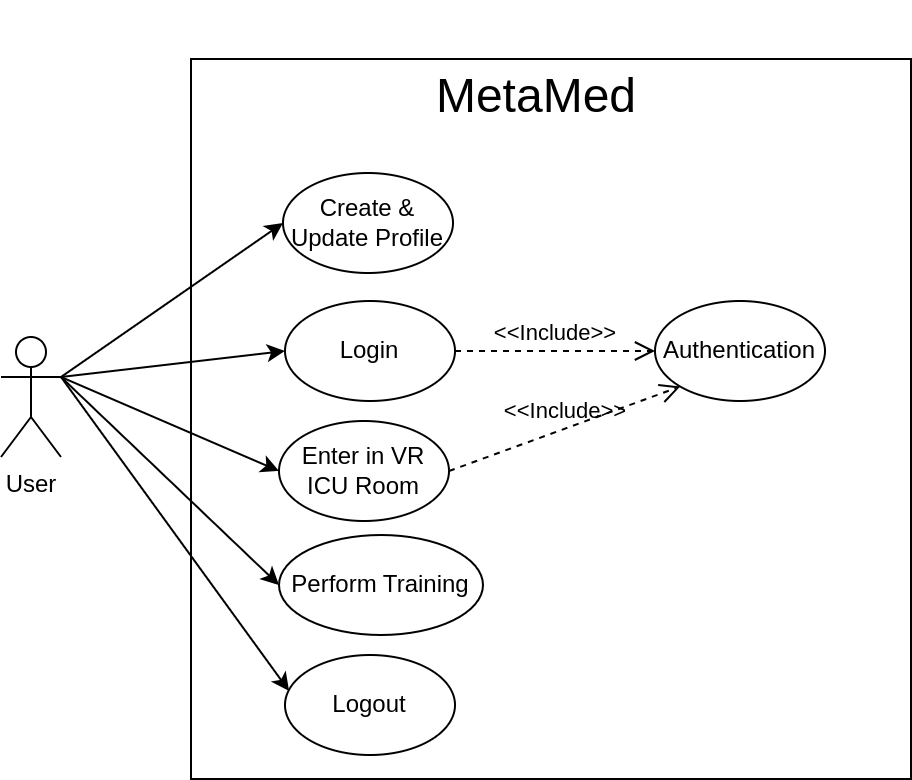
\includegraphics[width=0.5\textwidth, height=0.3\textheight]{Images/Use Case.drawio.png}
    \caption{Use Case Diagram}
    \label{fig:system-diagram}
\end{figure}

\section{System Diagram}
System Diagrams are visual representations of dynamic forces and interactions within a process, serving as more than just a process flow chart.
\begin{figure}[h]
    \centering
    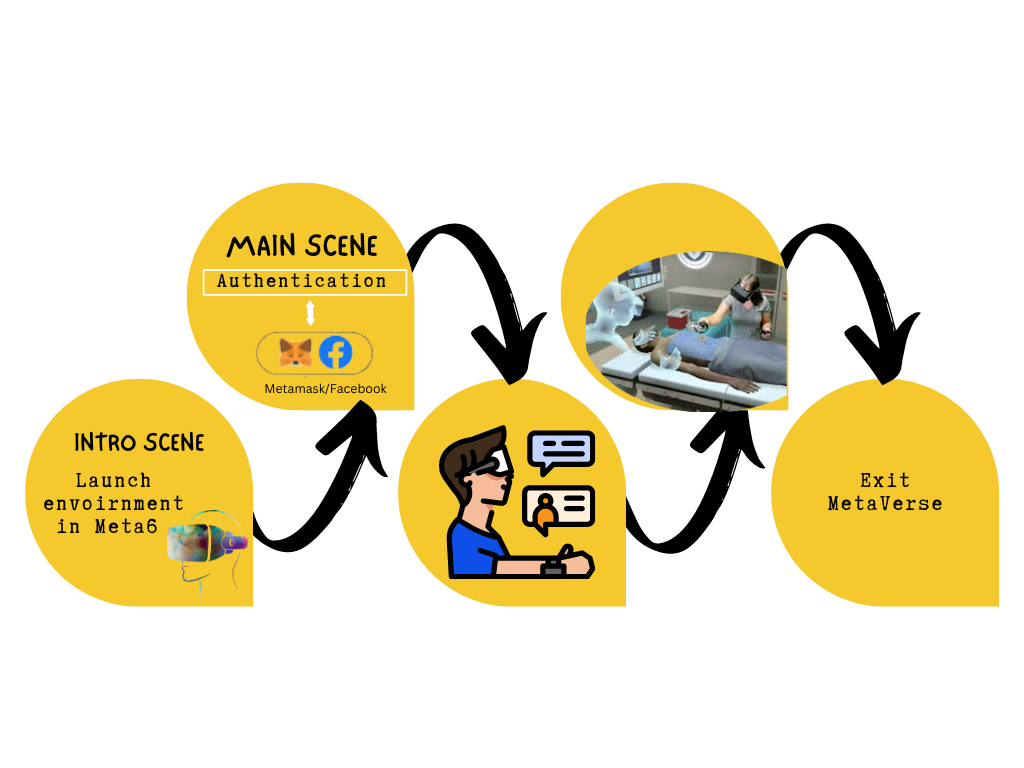
\includegraphics[width=0.7\textwidth, height=0.3\textheight]{Images/system.png}
    \caption{System Diagram}
    \label{fig:system-diagram}
\end{figure}


\section{Activity Diagram}
Activity diagrams are visual representations of a system's behavior, used to model various systems and processes, including business workflows, software systems, and organizational processes.
\begin{figure}[h]
    \centering
    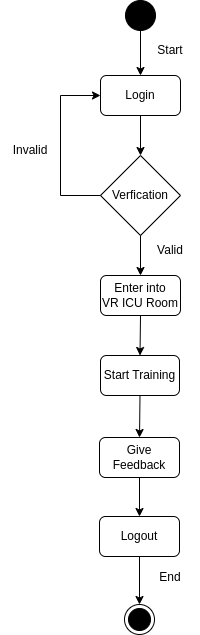
\includegraphics[width=0.3\textwidth, height=0.6\textheight]{Images/Activity.drawio.png}
    \caption{Activity Diagram}
    \label{fig:system-diagram}
\end{figure}
	\chapter{Iteration Plan 2 (FYP 1 Final)}
\label{ch:iter2}
This chapter outlines the second iteration plan for our project, providing guidance on module development and addressing students' discussion on the second stage of implementation method.

\section{FYP 1 Final:}
\begin{itemize}
    \item FYP 1 Final Presentation: \begin{itemize}
    \item Environment setup in Unity3D and Blender 
    \item Designed basic environment of Hospital
    \end{itemize}
\end{itemize}

\section{Designed basic environment of Hospital:}
	\begin{itemize}
	\item Reception Area
	\item Waiting Rooms
	\item Patient Rooms
	\item Training Facilities
\end{itemize}	
	
\subsection{Hospital Entrance:}
The hospital entrance serves as the main entry point to the virtual hospital
	\begin{figure}[h]
		\centering
		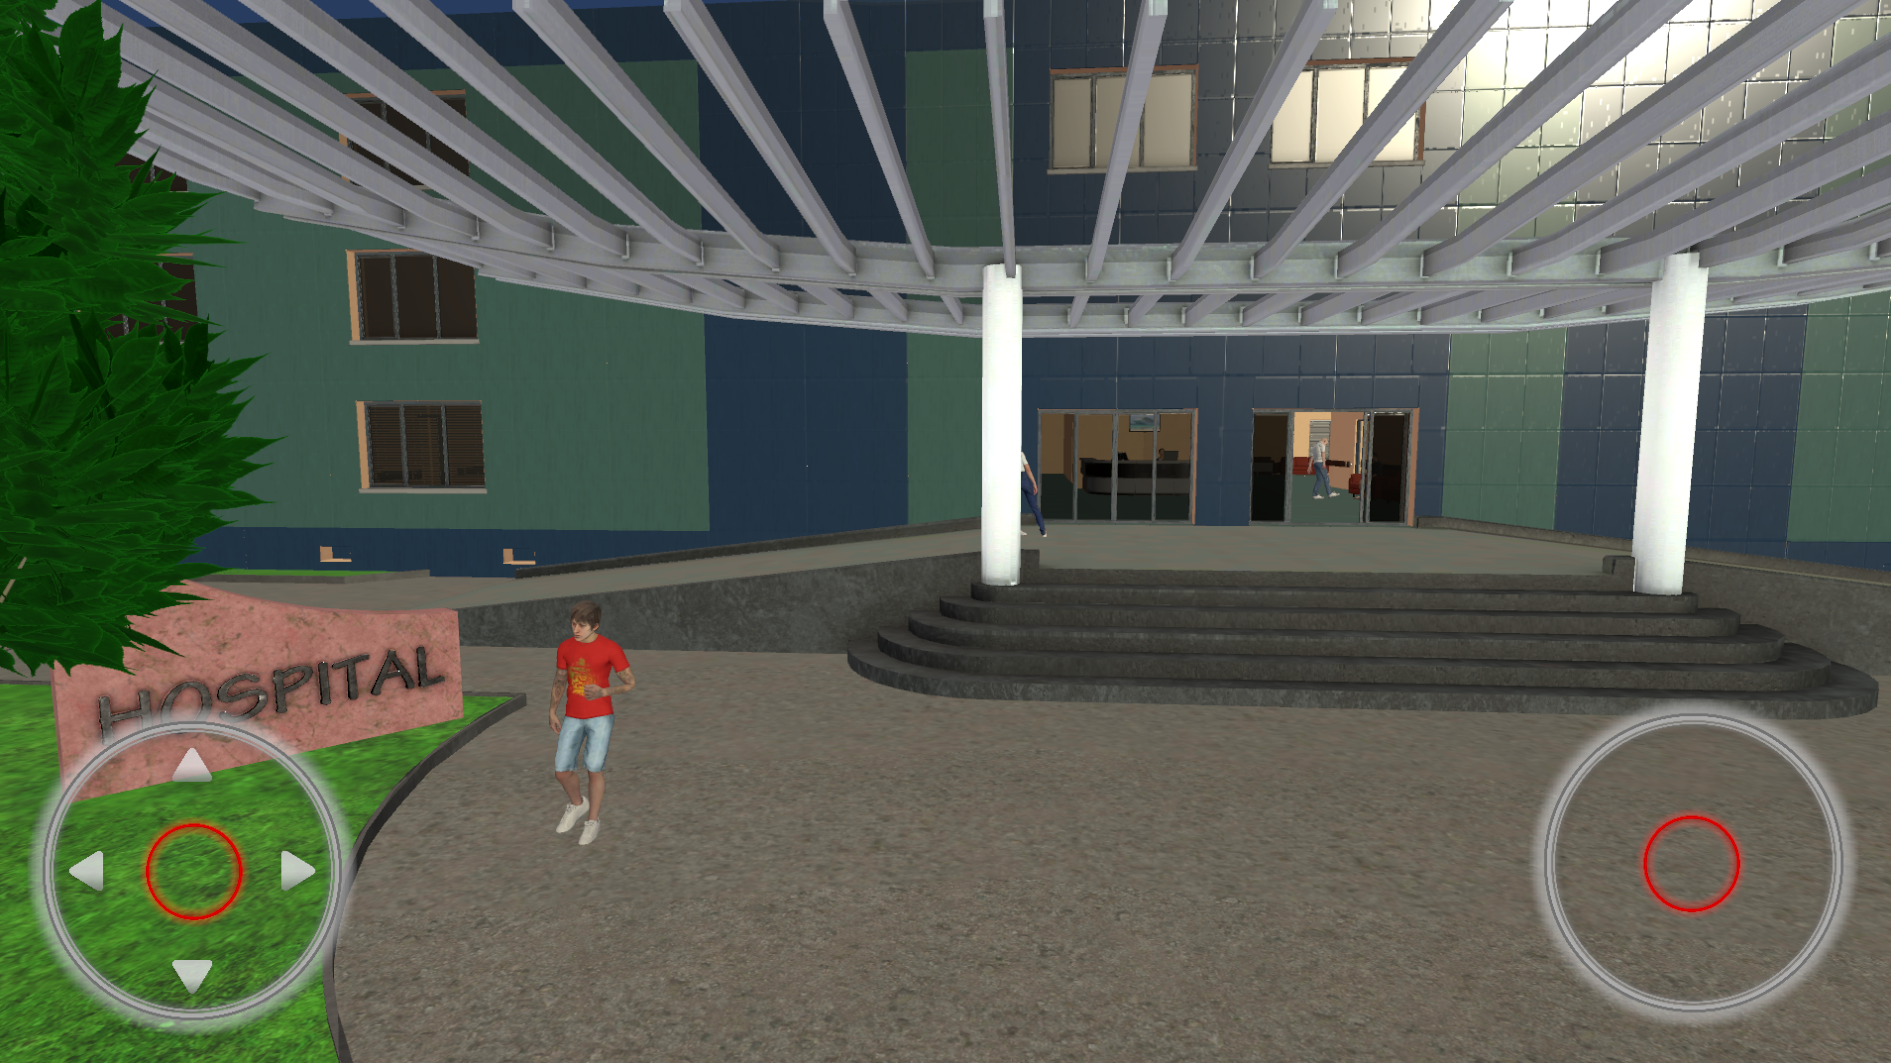
\includegraphics[width=0.7\textwidth, height=0.3\textheight]{Images/Hospital Enterance.png}
		\caption{Hospital Enterance}
		\label{fig:system-diagram}
	\end{figure}
\newline

\subsection{Reception Area:}
The reception area is the primary entrance to the virtual hospital, where patients and visitors can check-in and provide necessary information.
\begin{figure}[h]
	\centering
	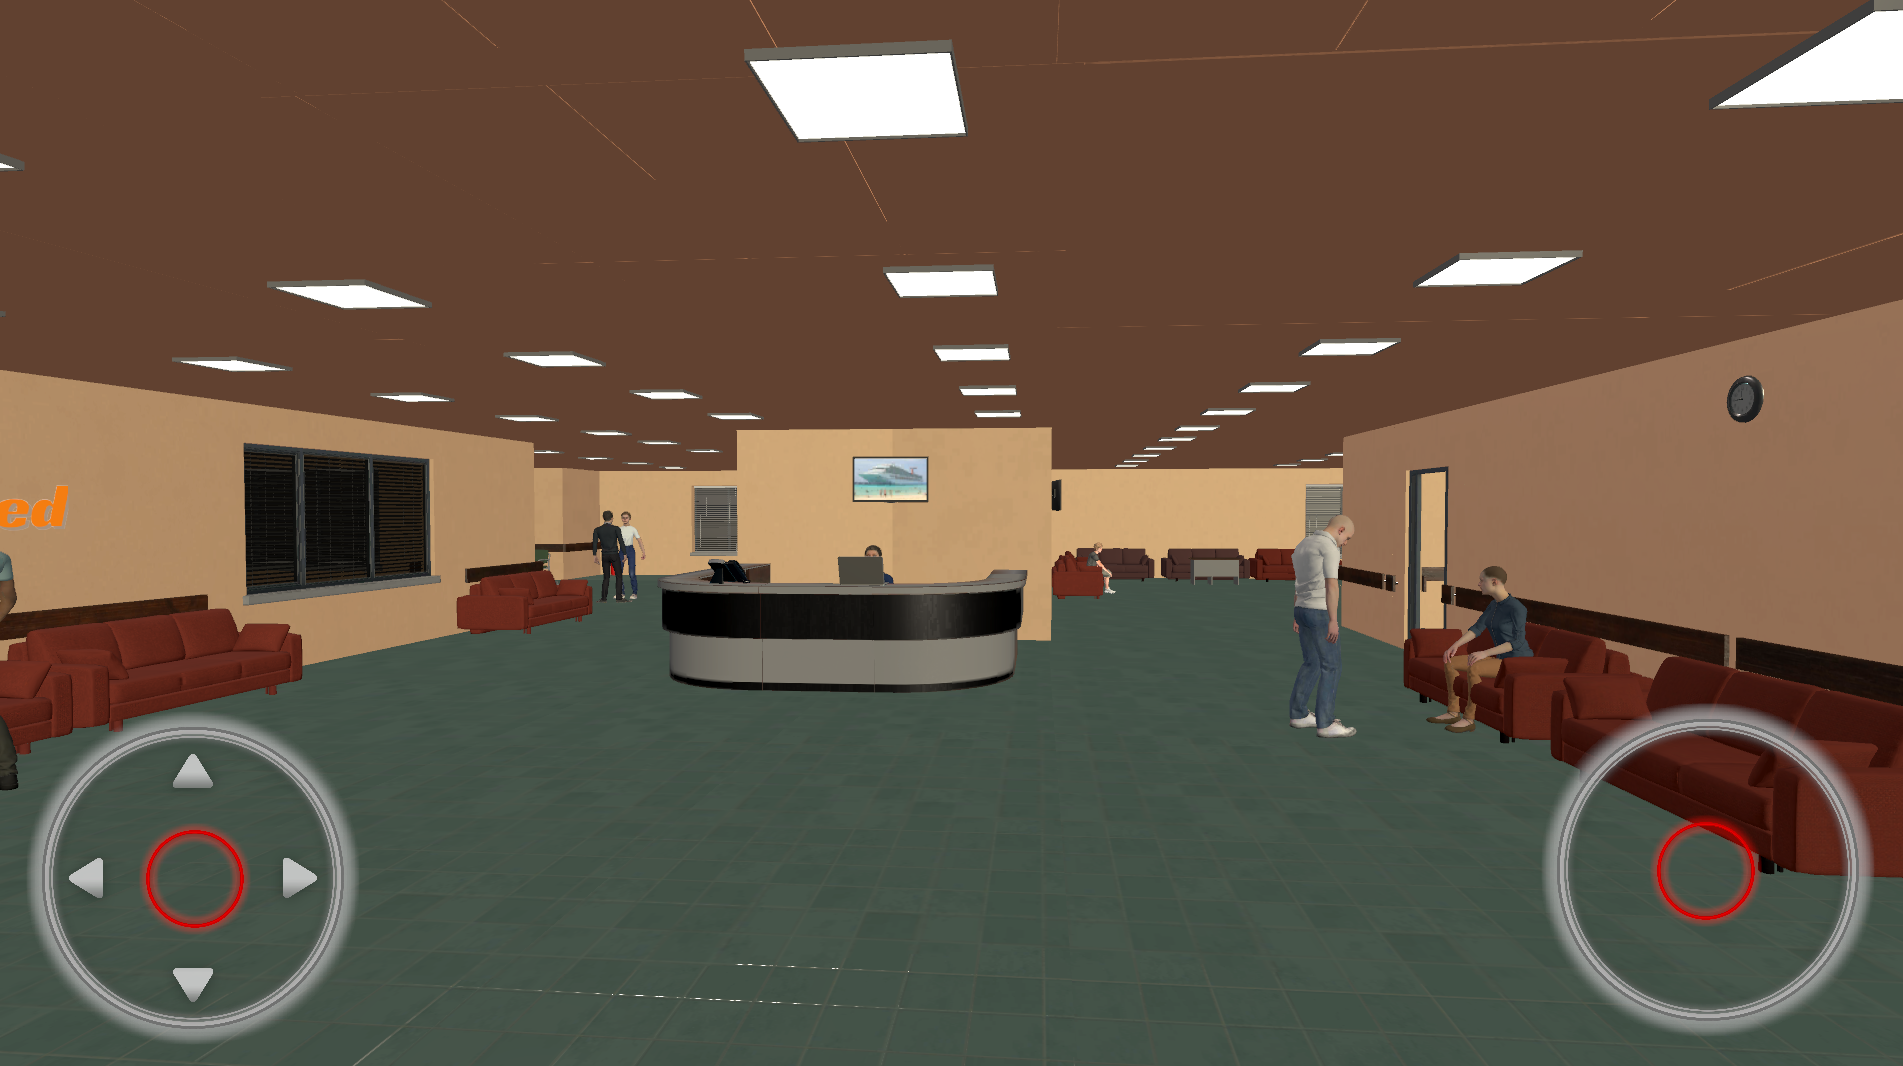
\includegraphics[width=0.7\textwidth, height=0.3\textheight]{Images/Reception Area.png}
	\caption{Reception Area}
	\label{fig:Reception Area}
\end{figure}
\newline

\subsection{Waiting Area:}	
Waiting area is designed to provide comfortable seating arrangements for patients and their companions while they wait for appointments or procedures.
\begin{figure}[h]
		\centering
		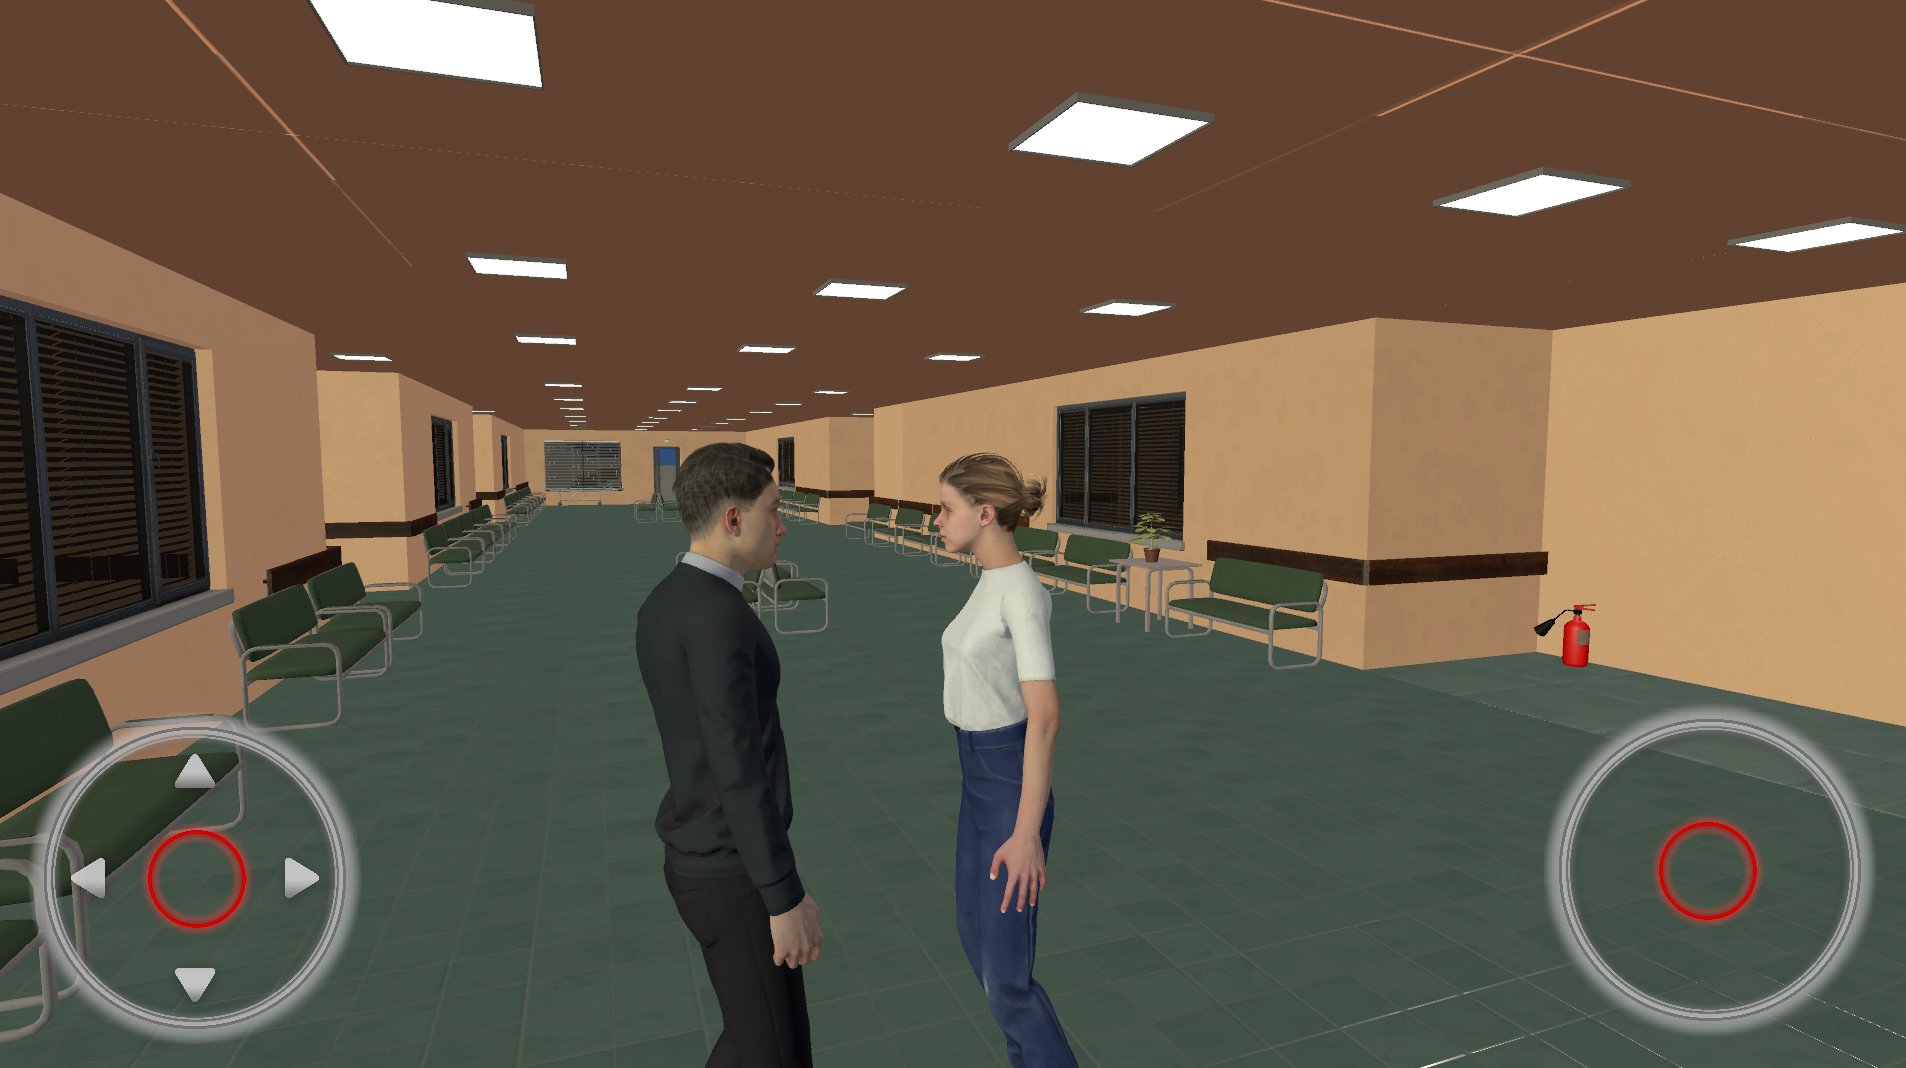
\includegraphics[width=0.7\textwidth, height=0.3\textheight]{Images/Waiting Area.png}
		\caption{Waiting Area}
\end{figure}
\\
\subsection{Patient Rooms:}	
Patient rooms are designed to offer a comfortable and healing atmosphere for patients during their hospital stay.
	\begin{figure}[h]
		\centering
		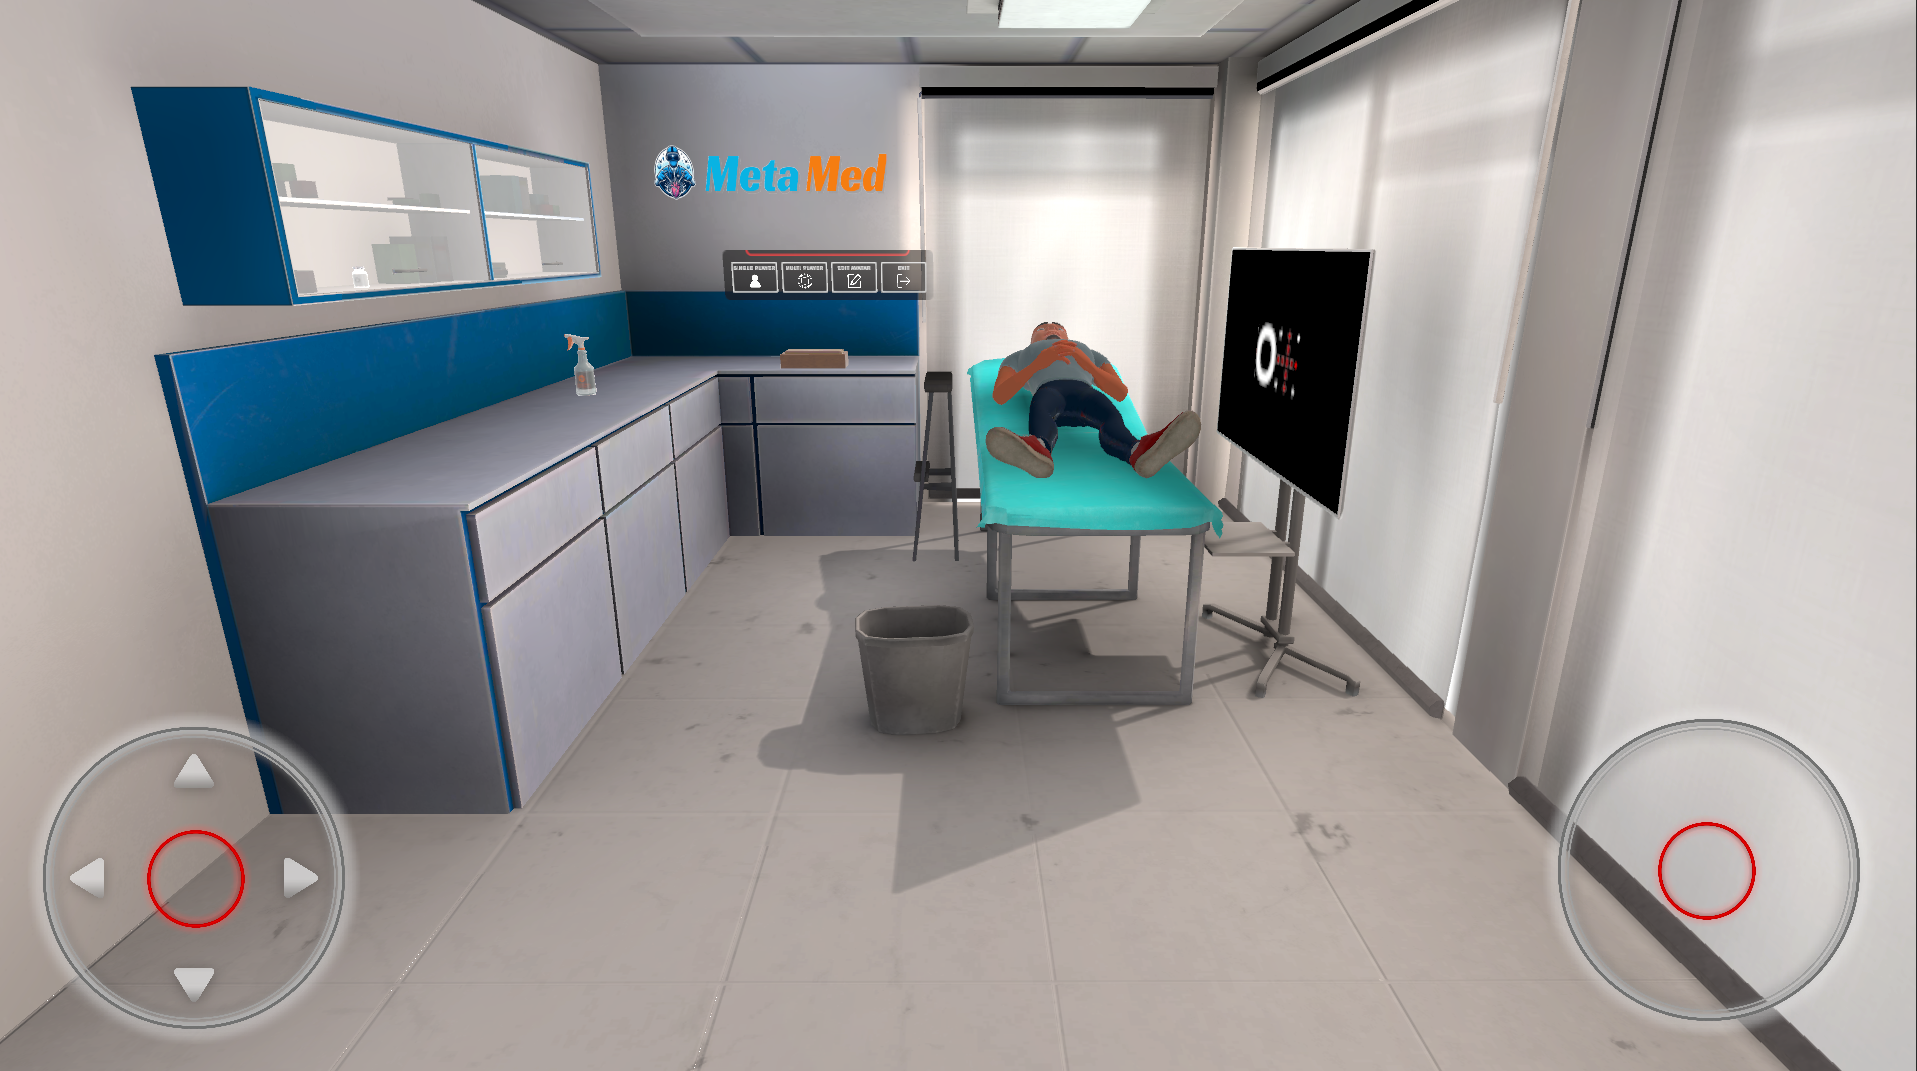
\includegraphics[width=0.7\textwidth, height=0.3\textheight]{Images/Patient Room.png}
		\caption{Patient Room}
		\label{fig:Patient-Room}
	\end{figure}	

\subsection{Patient Body:}	
Meta-verse Hospital has developed Patient Body to simulate patient interactions, offer realistic medical scenarios for training, and enhance healthcare professionals' virtual learning experiences.
\begin{figure}[h]
	\centering
	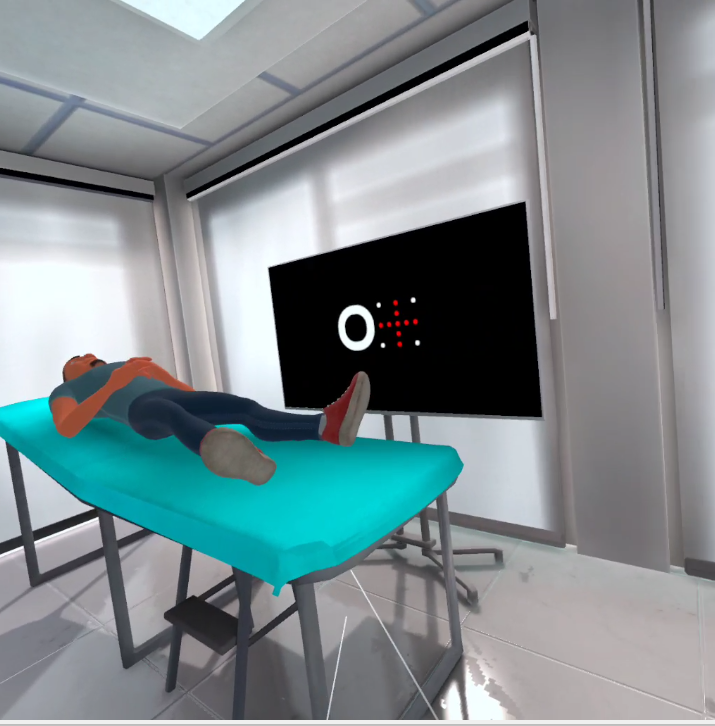
\includegraphics[width=0.7\textwidth, height=0.3\textheight]{Images/Patient Body.png}
	\caption{Patient Room}
	\label{fig:Patient Room}
\end{figure}	

	
	\chapter{Iteration 3 (FYP-2 Mid)}
\label{ch:iter3}
The first iteration is expected to be completed by the midterm of the FYP-2.
This chapter will have some of the artifacts based on system design. The requirements analysis section is same for all the systems while the design may vary. There may have two types of designs the structural design or . First section is for the structural design.
\section{FYP-2 Mid}
\textbf{Objectives for FYP-2 Mid}
	\begin{itemize}
		\item Basic tools
		\item Medicines 
		\item User movements
		\item Grabbing Tools
	\end{itemize}
\newpage
\subsection{Tools and Medicines}
\begin{figure}[h]
	\centering
	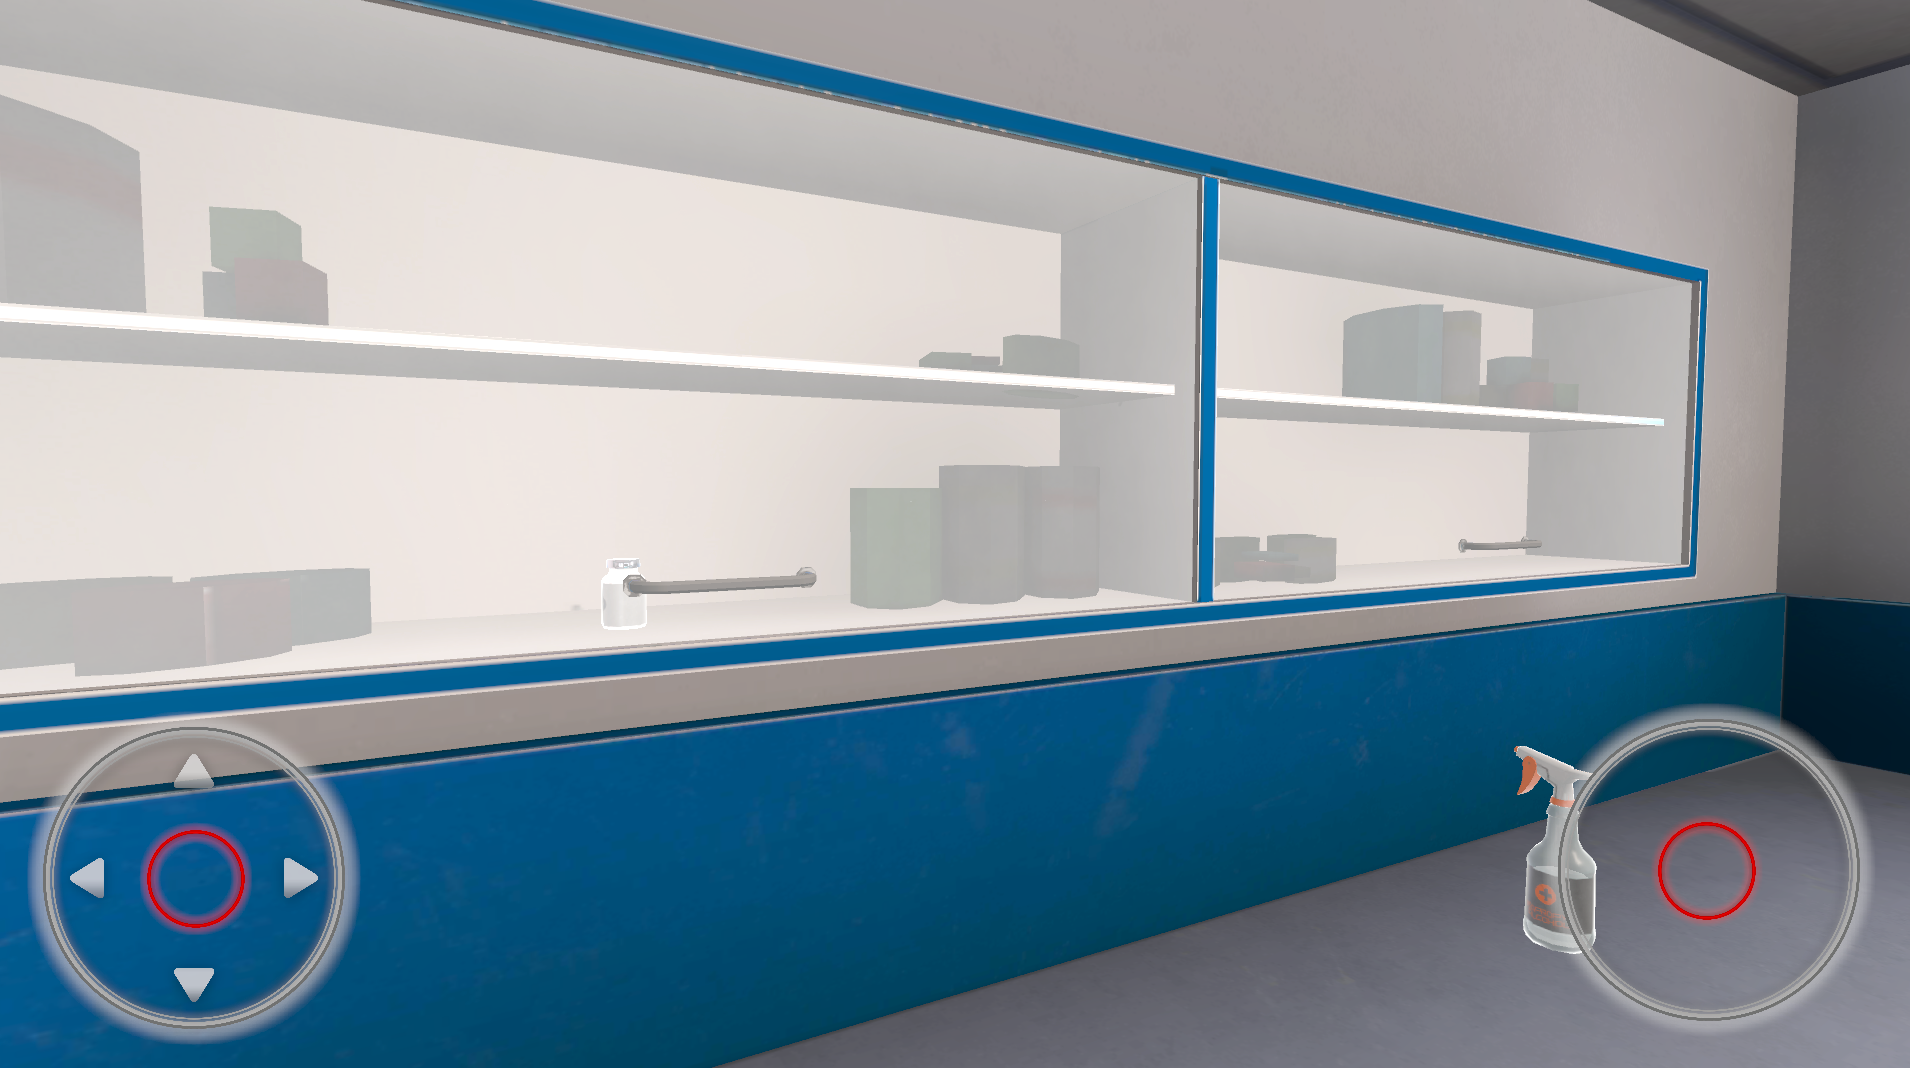
\includegraphics[width=0.7\textwidth, height=0.3\textheight]{Images/Tools and Medicine.png}
	\caption{Tools and Medicine box}
	\label{fig:Tools and Medicine}
\end{figure}

\subsection{Tools Grabbing}
\begin{figure}[h]
	\centering
	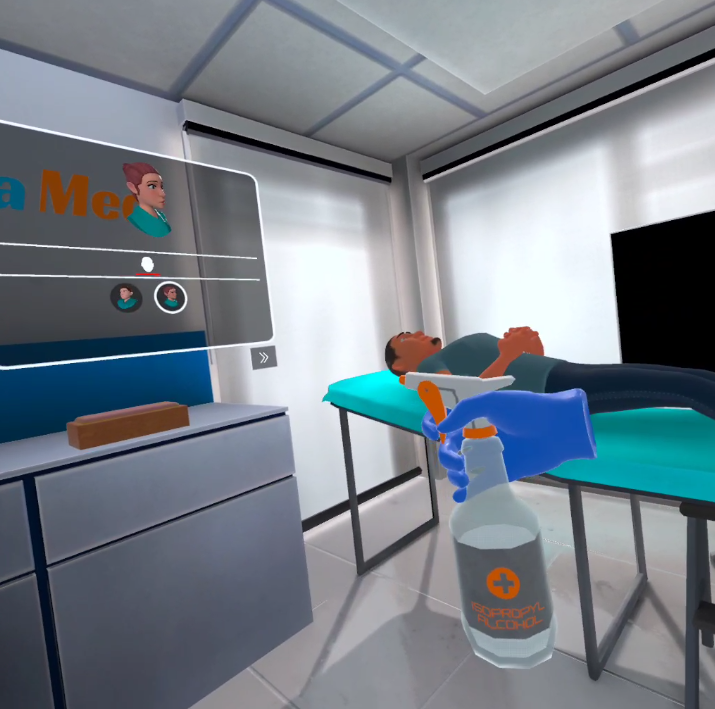
\includegraphics[width=0.7\textwidth, height=0.3\textheight]{Images/Grabbing Tool.png}
	\caption{Grabbing Tools}
	\label{fig:Grabbing Tools}
\end{figure}
\newpage
\subsubsection{Hands Washing}
\text{Here we are washing hand.}
\begin{figure}[h]
	\centering
     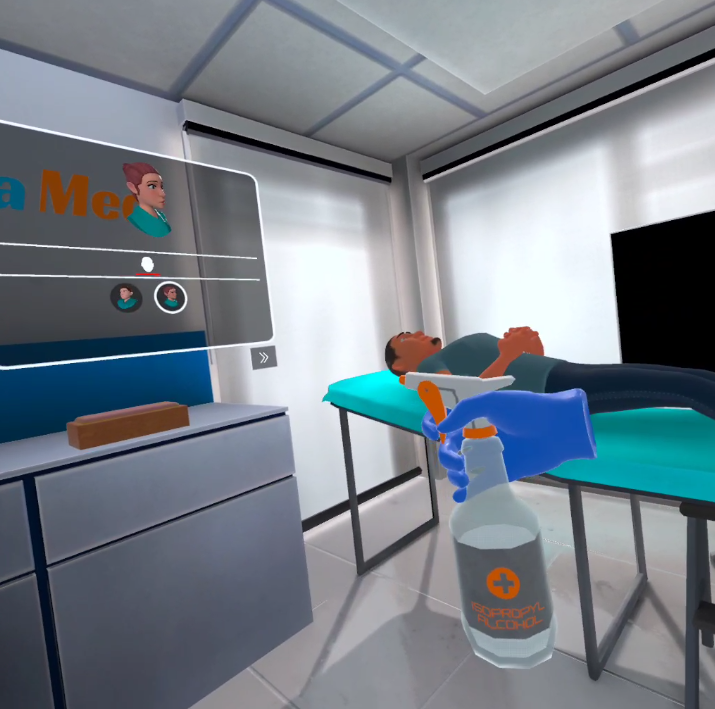
\includegraphics[width=0.7\textwidth, height=0.3\textheight]{Images/Washing hands.png}
	\caption{Hands Washing}
	\label{fig:Hands Washing}
\end{figure}

\subsubsection{Pour Alcohol}
\text{Here we are pouring alcohol to on cotton bud.}
\begin{figure}[h]
	\centering
	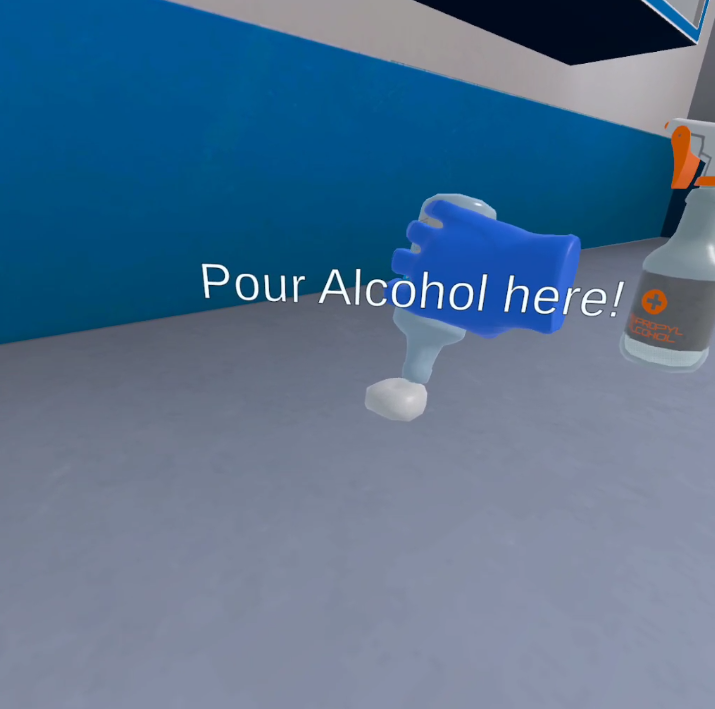
\includegraphics[width=0.7\textwidth, height=0.3\textheight]{Images/Pour Alcohol.png}
	\caption{Pour Alcohol}
	\label{fig:Pour-Alcohol}
\end{figure}
\newpage
\subsubsection{Clean the injection site}
\text{Here we are cleaning the injection site.}
\begin{figure}[h]
	\centering
	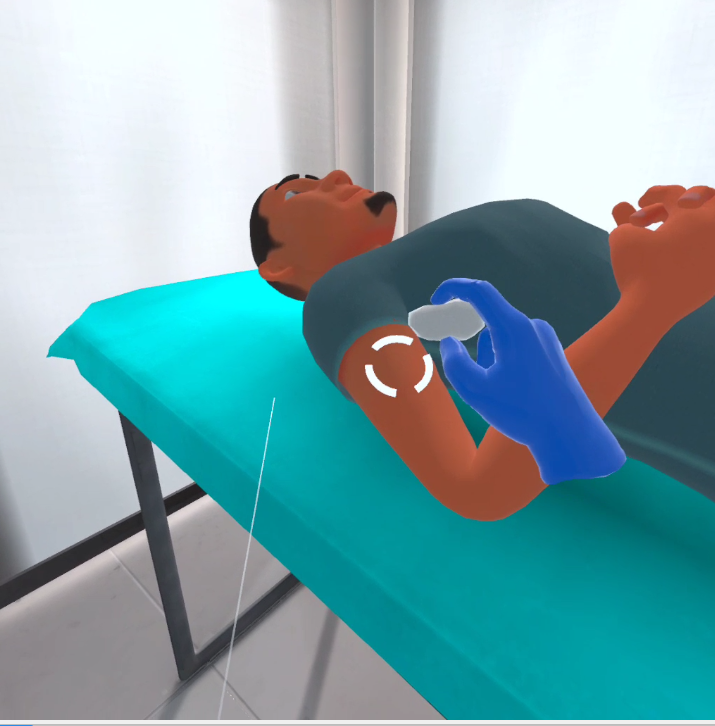
\includegraphics[width=0.7\textwidth, height=0.3\textheight]{Images/Clean the injection site.png}
	\caption{Clean the injection site}
	\label{fig:Clean the injection site}
\end{figure}
\subsubsection{Dispose the Cotton}
\text{Here we are disposing the cotton.}
\begin{figure}[h]
	\centering
	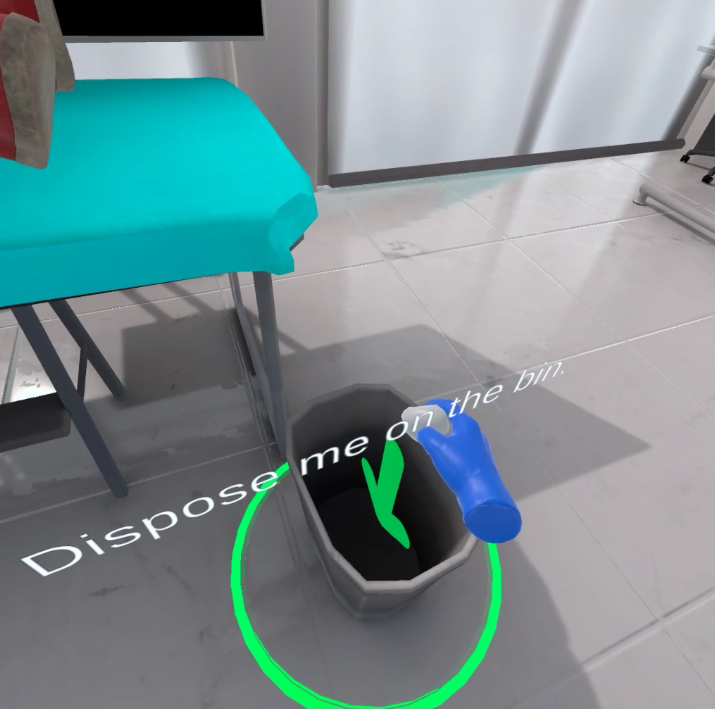
\includegraphics[width=0.7\textwidth, height=0.3\textheight]{Images/Dispose the Cotton.png}
	\caption{Dispose the Cotton}
	\label{fig:Dispose the Cotton}
\end{figure}
\newpage
\subsubsection{Picking the injection}
\text{Here we are picking the injection.}
\begin{figure}[h]
	\centering
	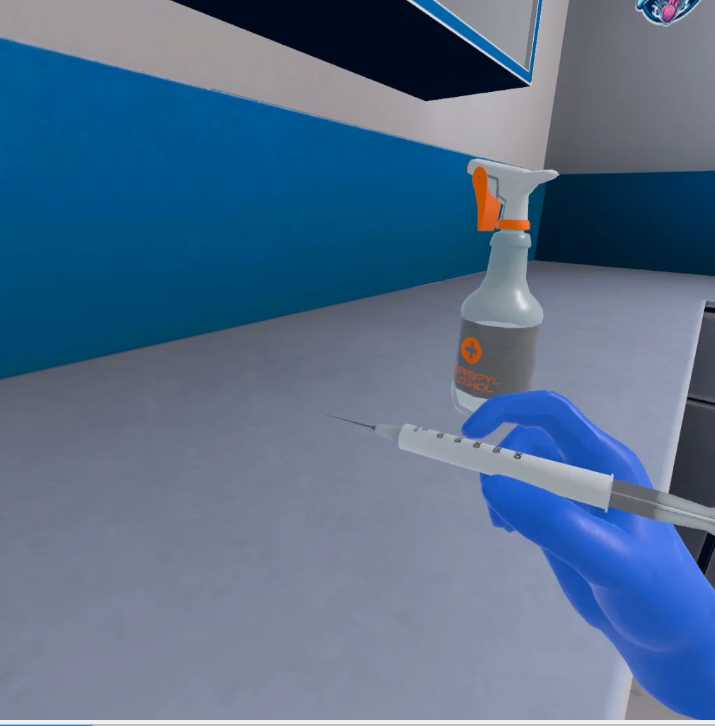
\includegraphics[width=0.7\textwidth, height=0.3\textheight]{Images/Picking the injection.png}
	\caption{Picking the injection}
	\label{fig:Picking the injection}
\end{figure}
\subsubsection{Inject the medication}
\text{Here we are inject the medication.}
\begin{figure}[h]
	\centering
	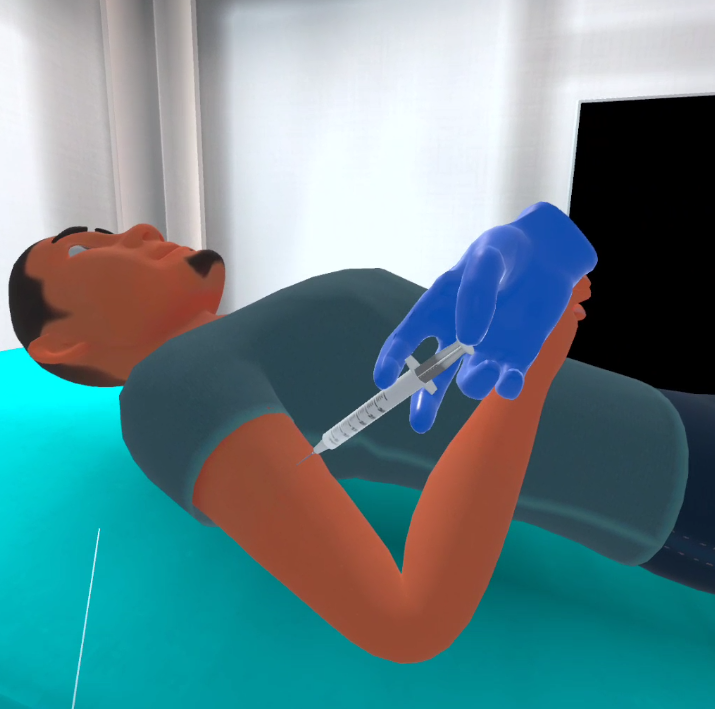
\includegraphics[width=0.7\textwidth, height=0.3\textheight]{Images/Inject the medication.png}
	\caption{Inject the medication}
	\label{fig:Inject the medication}
\end{figure}
\newpage
\subsubsection{Applying Cut on Body}
\text{Here we applying cut on body.}
\begin{figure}[h]
	\centering
	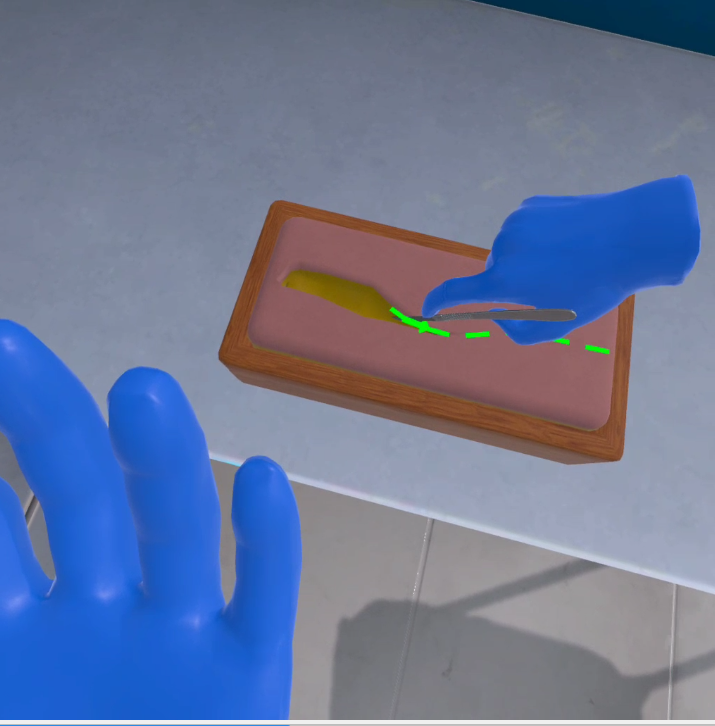
\includegraphics[width=0.7\textwidth, height=0.3\textheight]{Images/Applying Cut on Body.png}
	\caption{Applying Cut on Body}
	\label{fig:Applying Cut on Body}
\end{figure}
\newpage
\subsubsection{Objects Movement}
\text{Here are some code for actions performed by user.}
\text{User movement part 1 code.}
\newline
\begin{figure}[h]
	\centering
	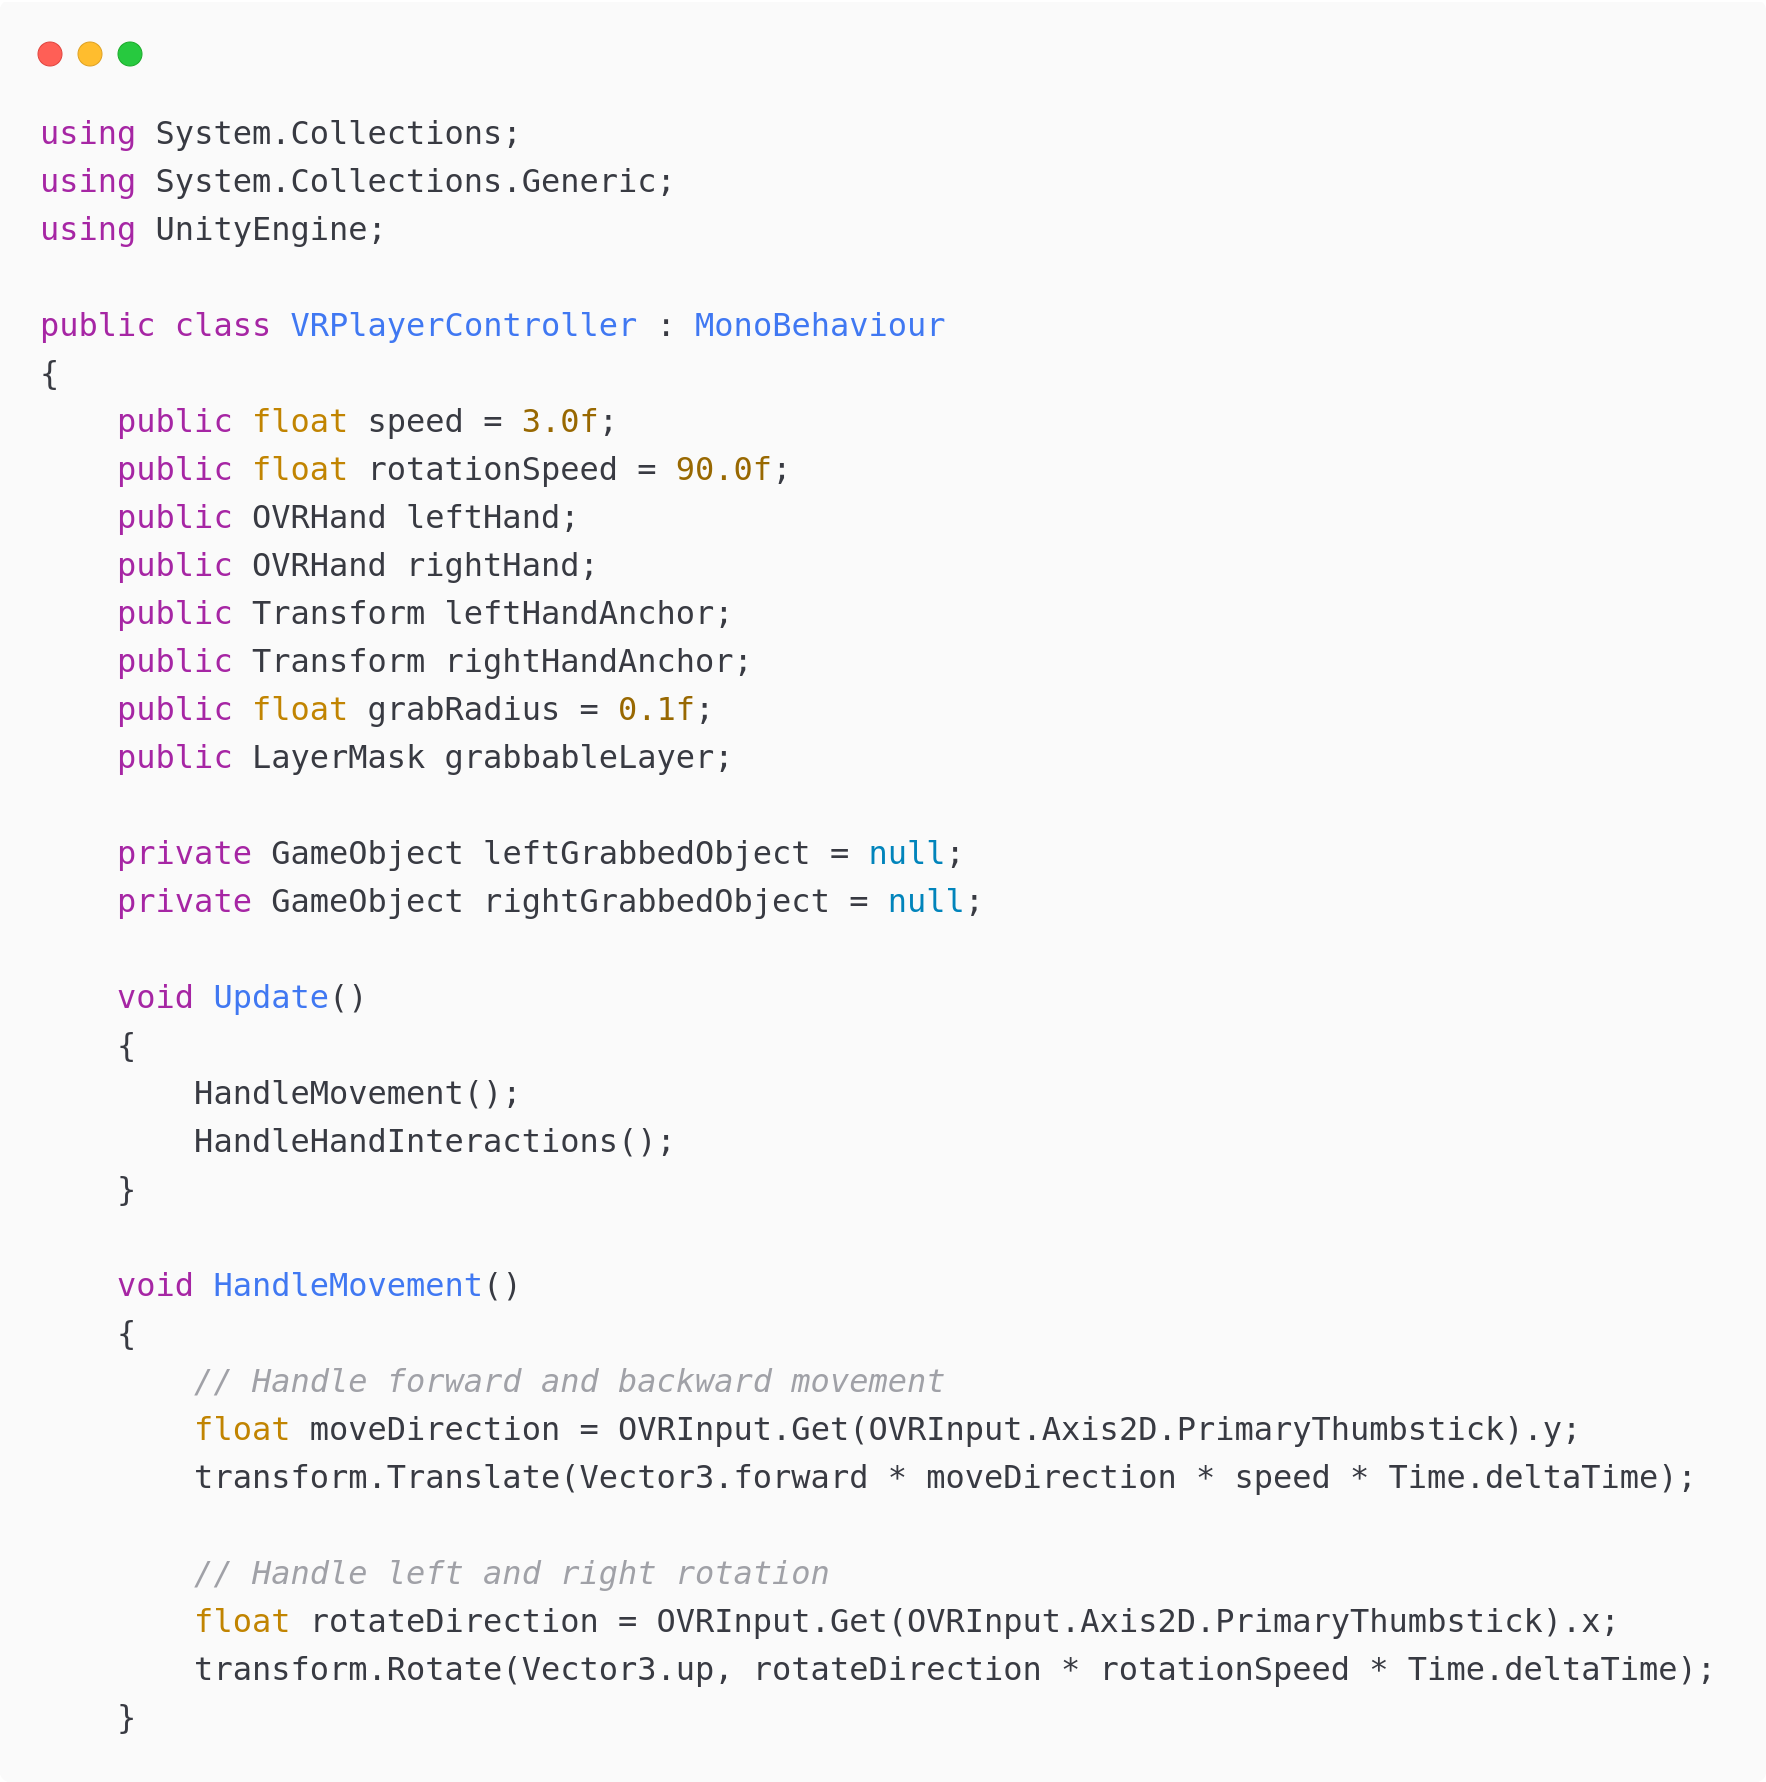
\includegraphics[width=1\textwidth, height=0.7\textheight]{Images/playerp1.png}
	\caption{User Movement Code 1}
	\label{User Movement Code 1}
\end{figure}
\newpage
\text{User movement part 2 code.}
\newline
\begin{figure}[h] 
	\centering
	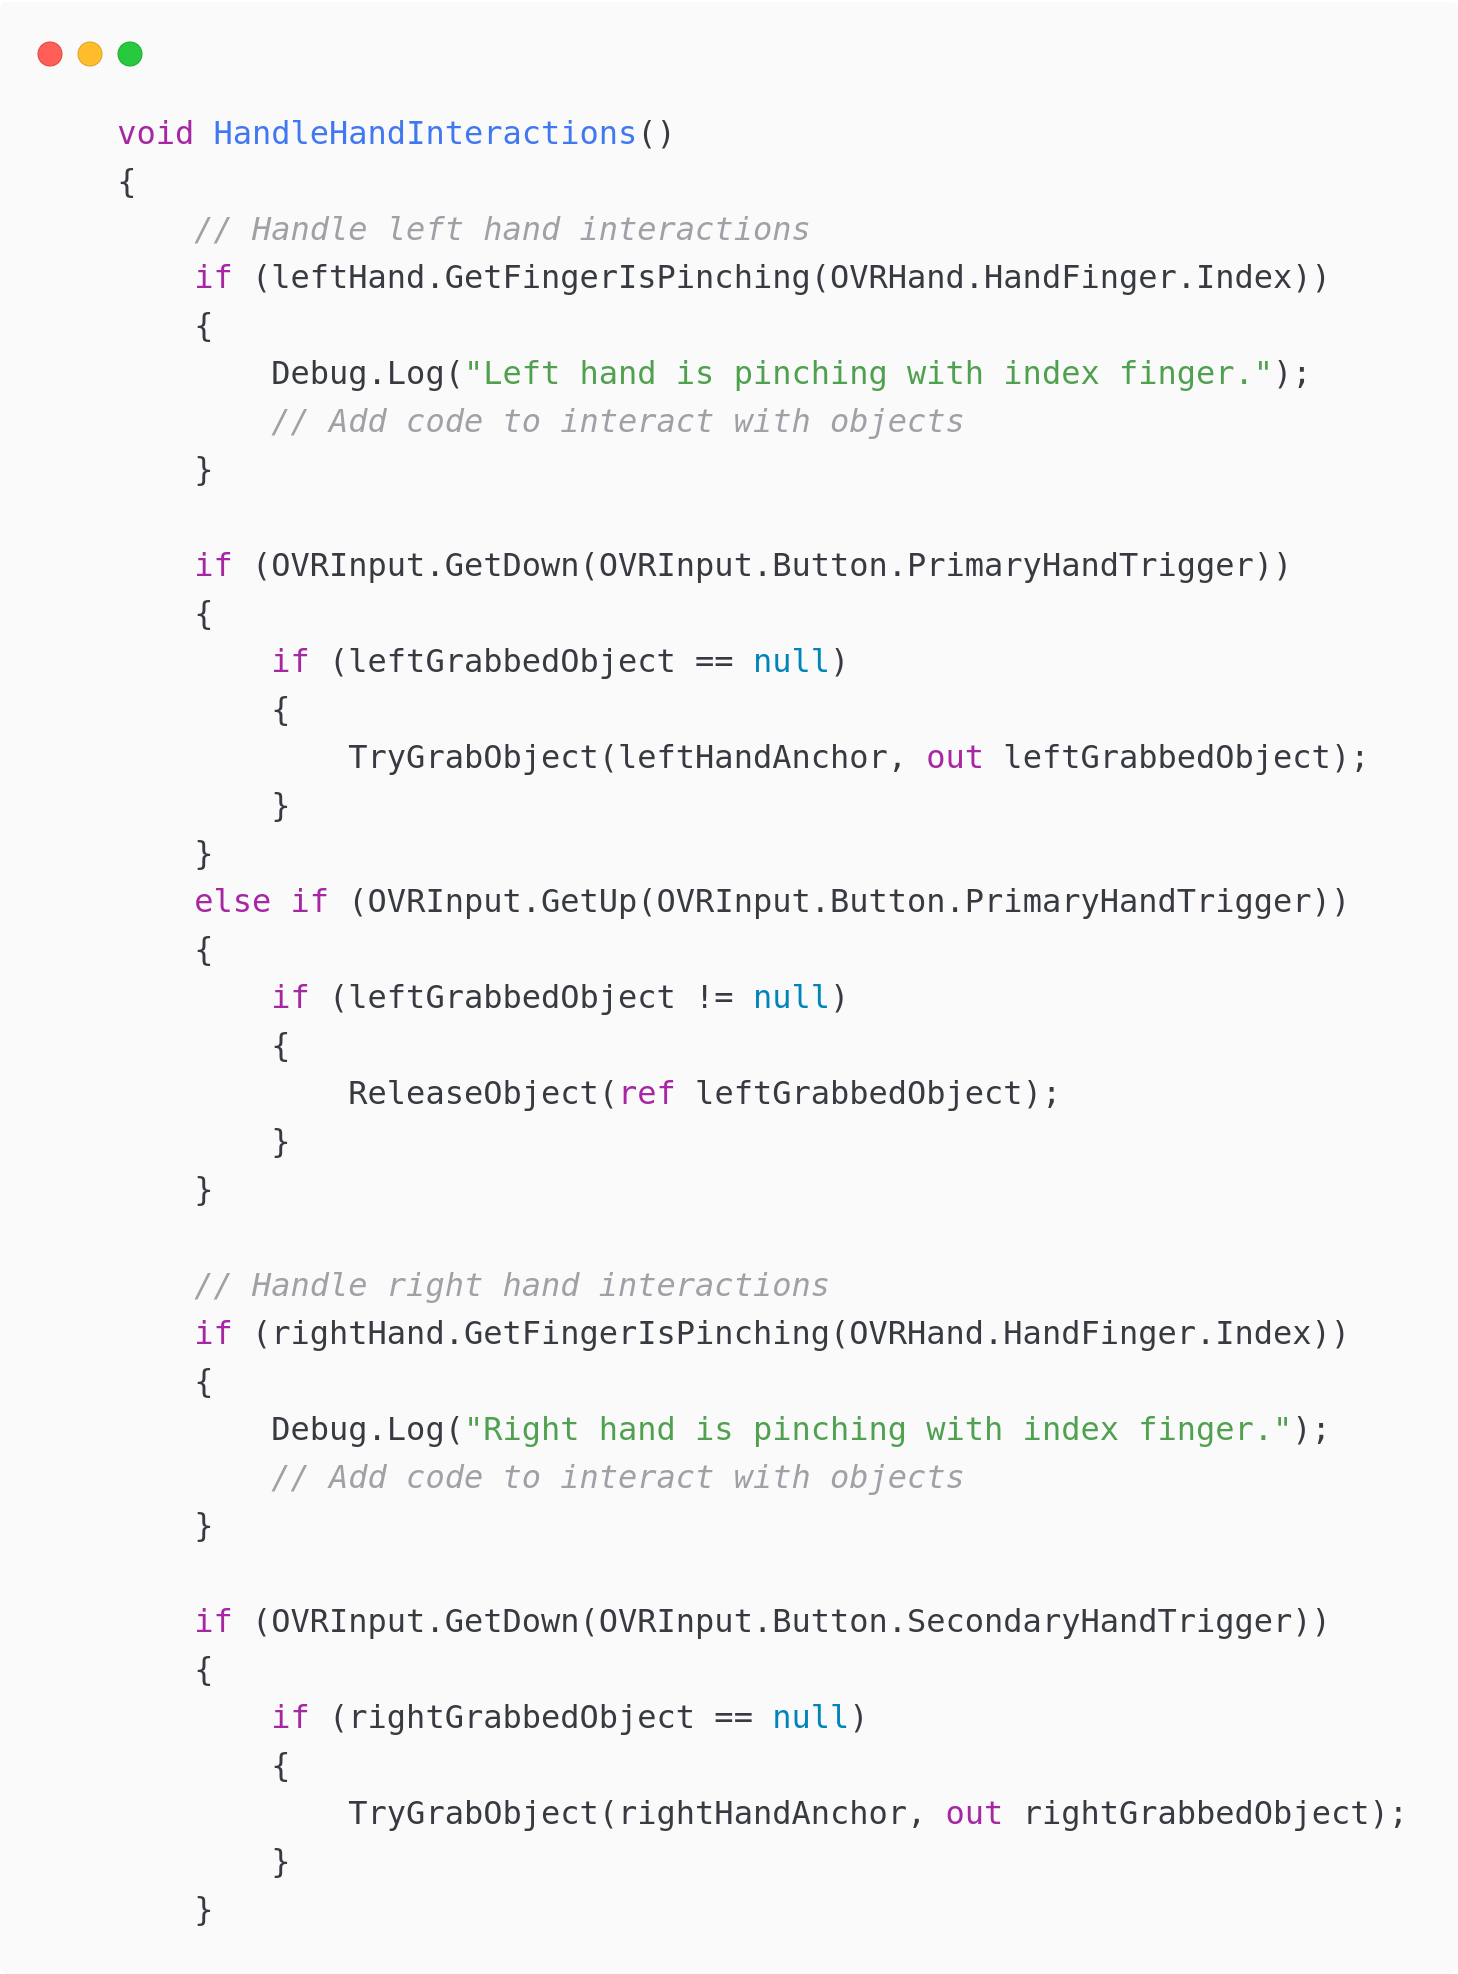
\includegraphics[width=1\textwidth, height=0.7\textheight]{Images/playerp2.png}
	\caption{User Movement Code 2}
	\label{fig:User Movement Code 2}
\end{figure}
\newpage
\text{User movement part 3 code.}
\newline
\begin{figure}[h] 
	\centering
	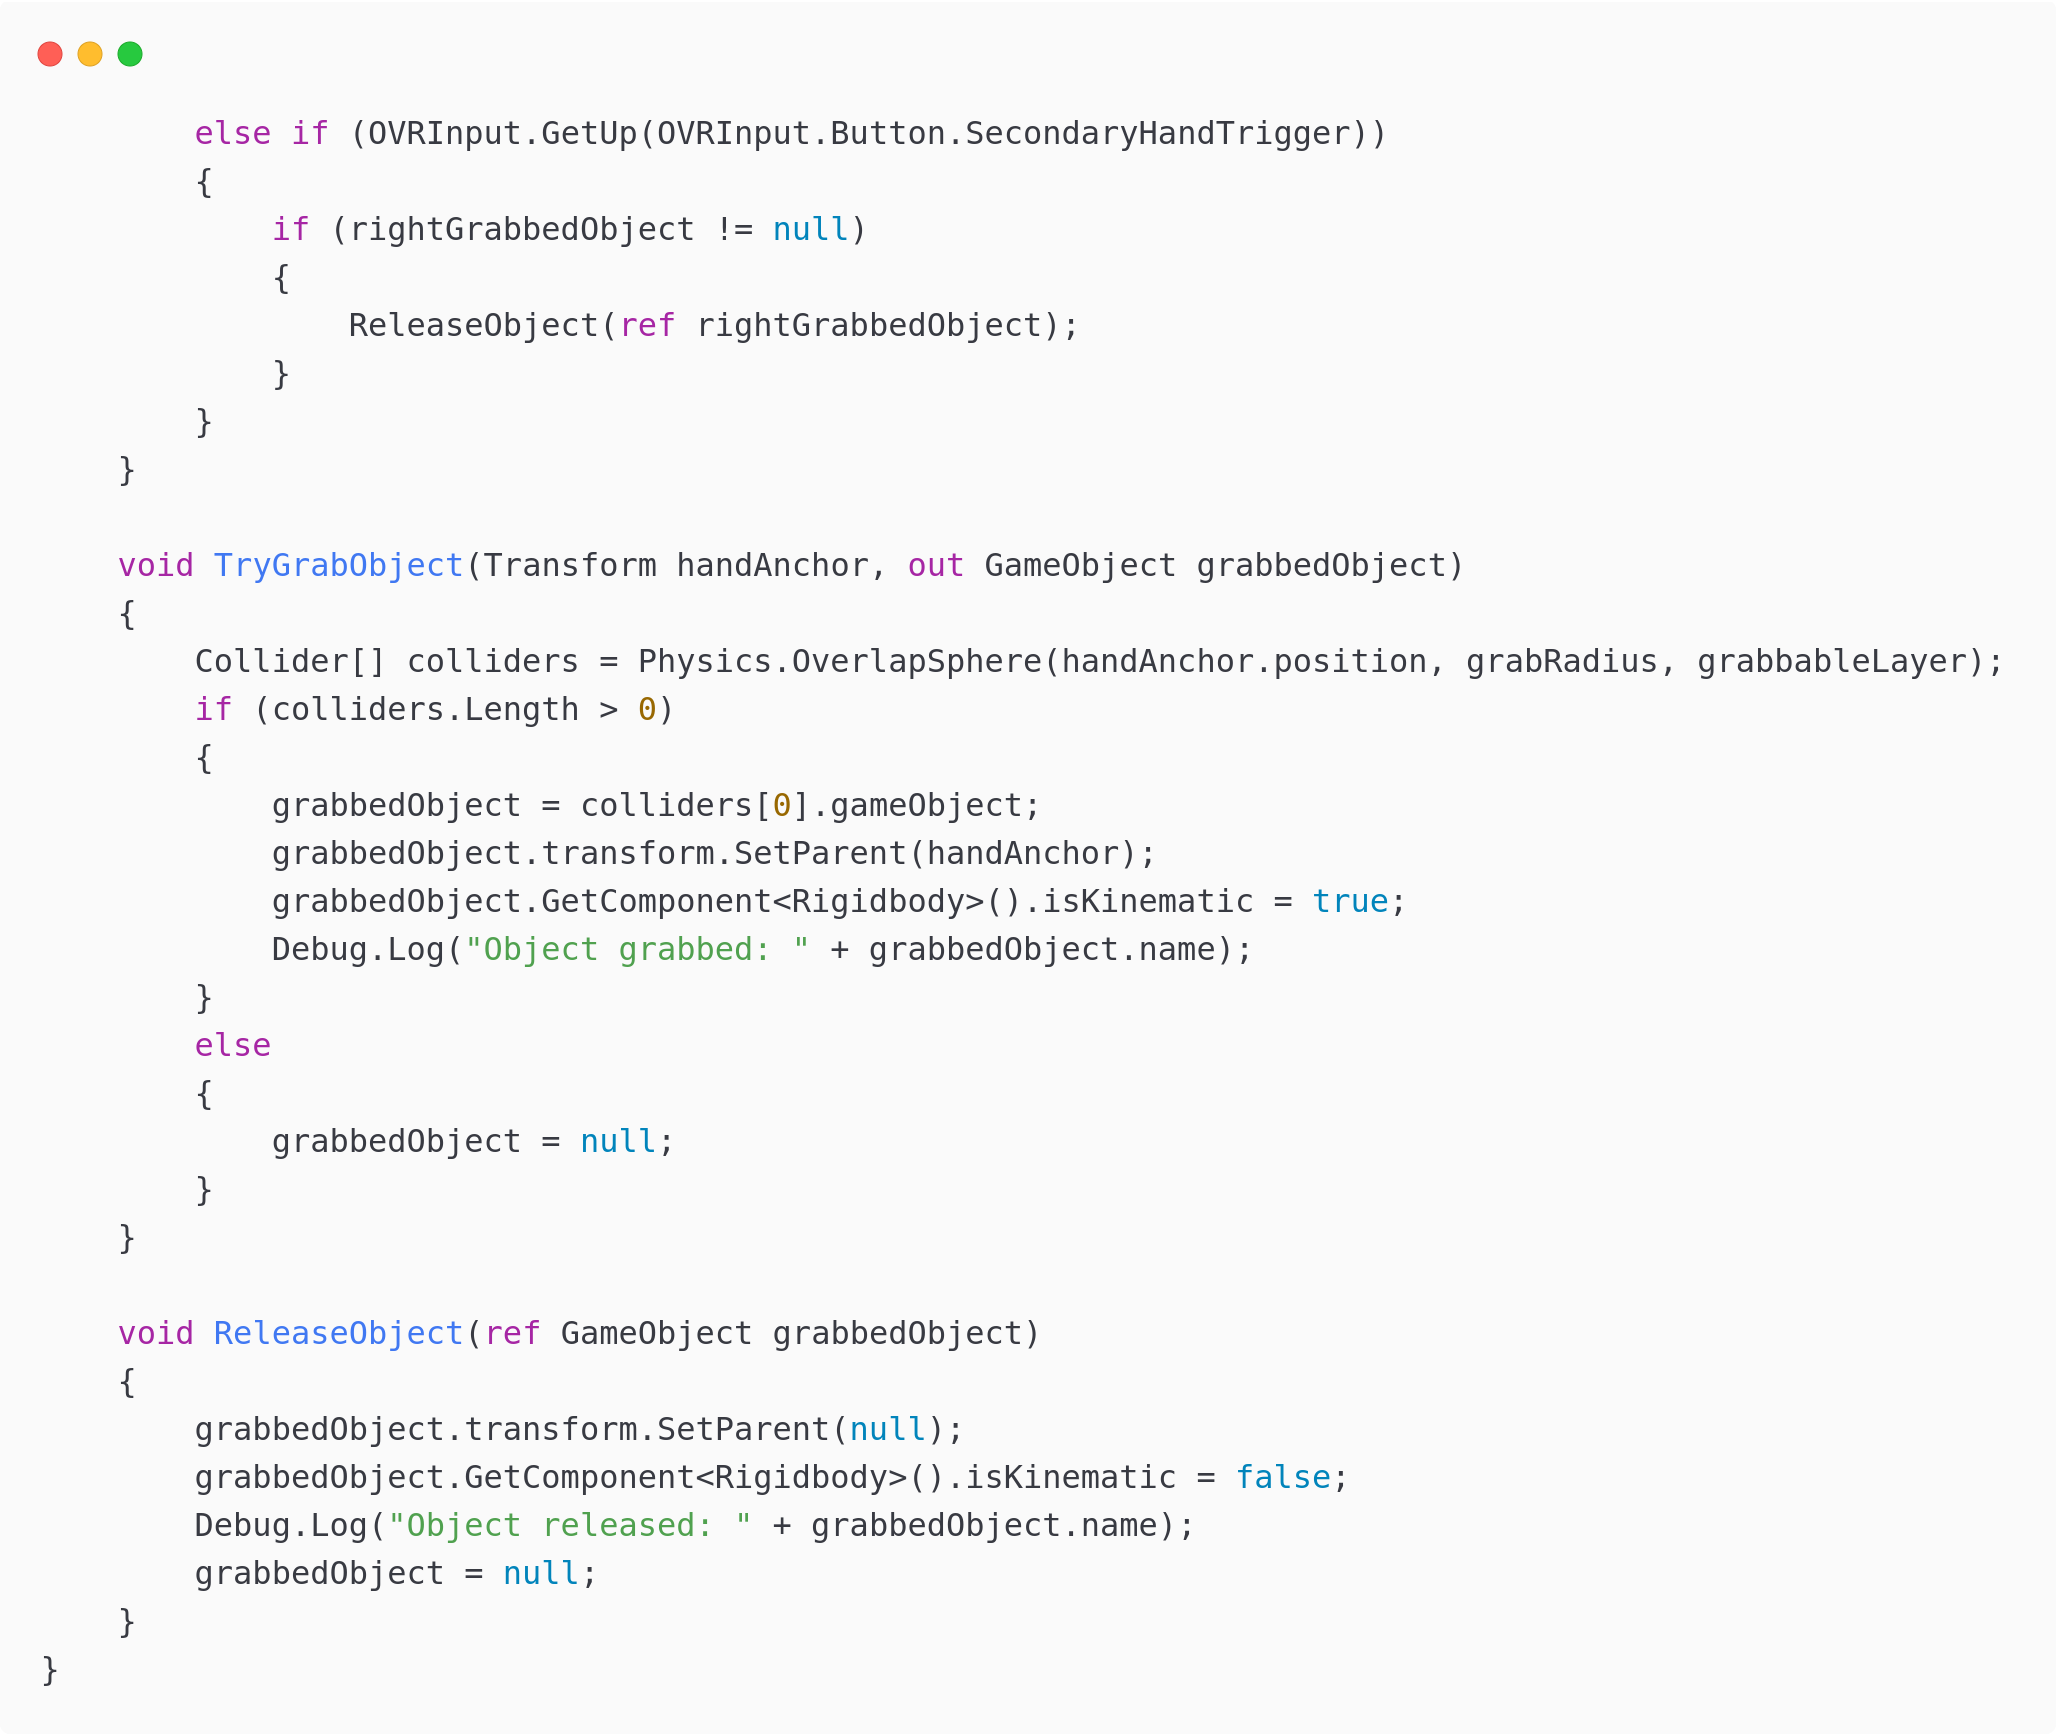
\includegraphics[width=1\textwidth, height=0.7\textheight]{Images/playerp3.png}
	\caption{User Movement Code 3}
	\label{fig:User Movement Code 3}
\end{figure}
\newpage
\text{Code for Pore Alcohol for Hands Washing.}
\newline
\begin{figure}[h]
	\centering
	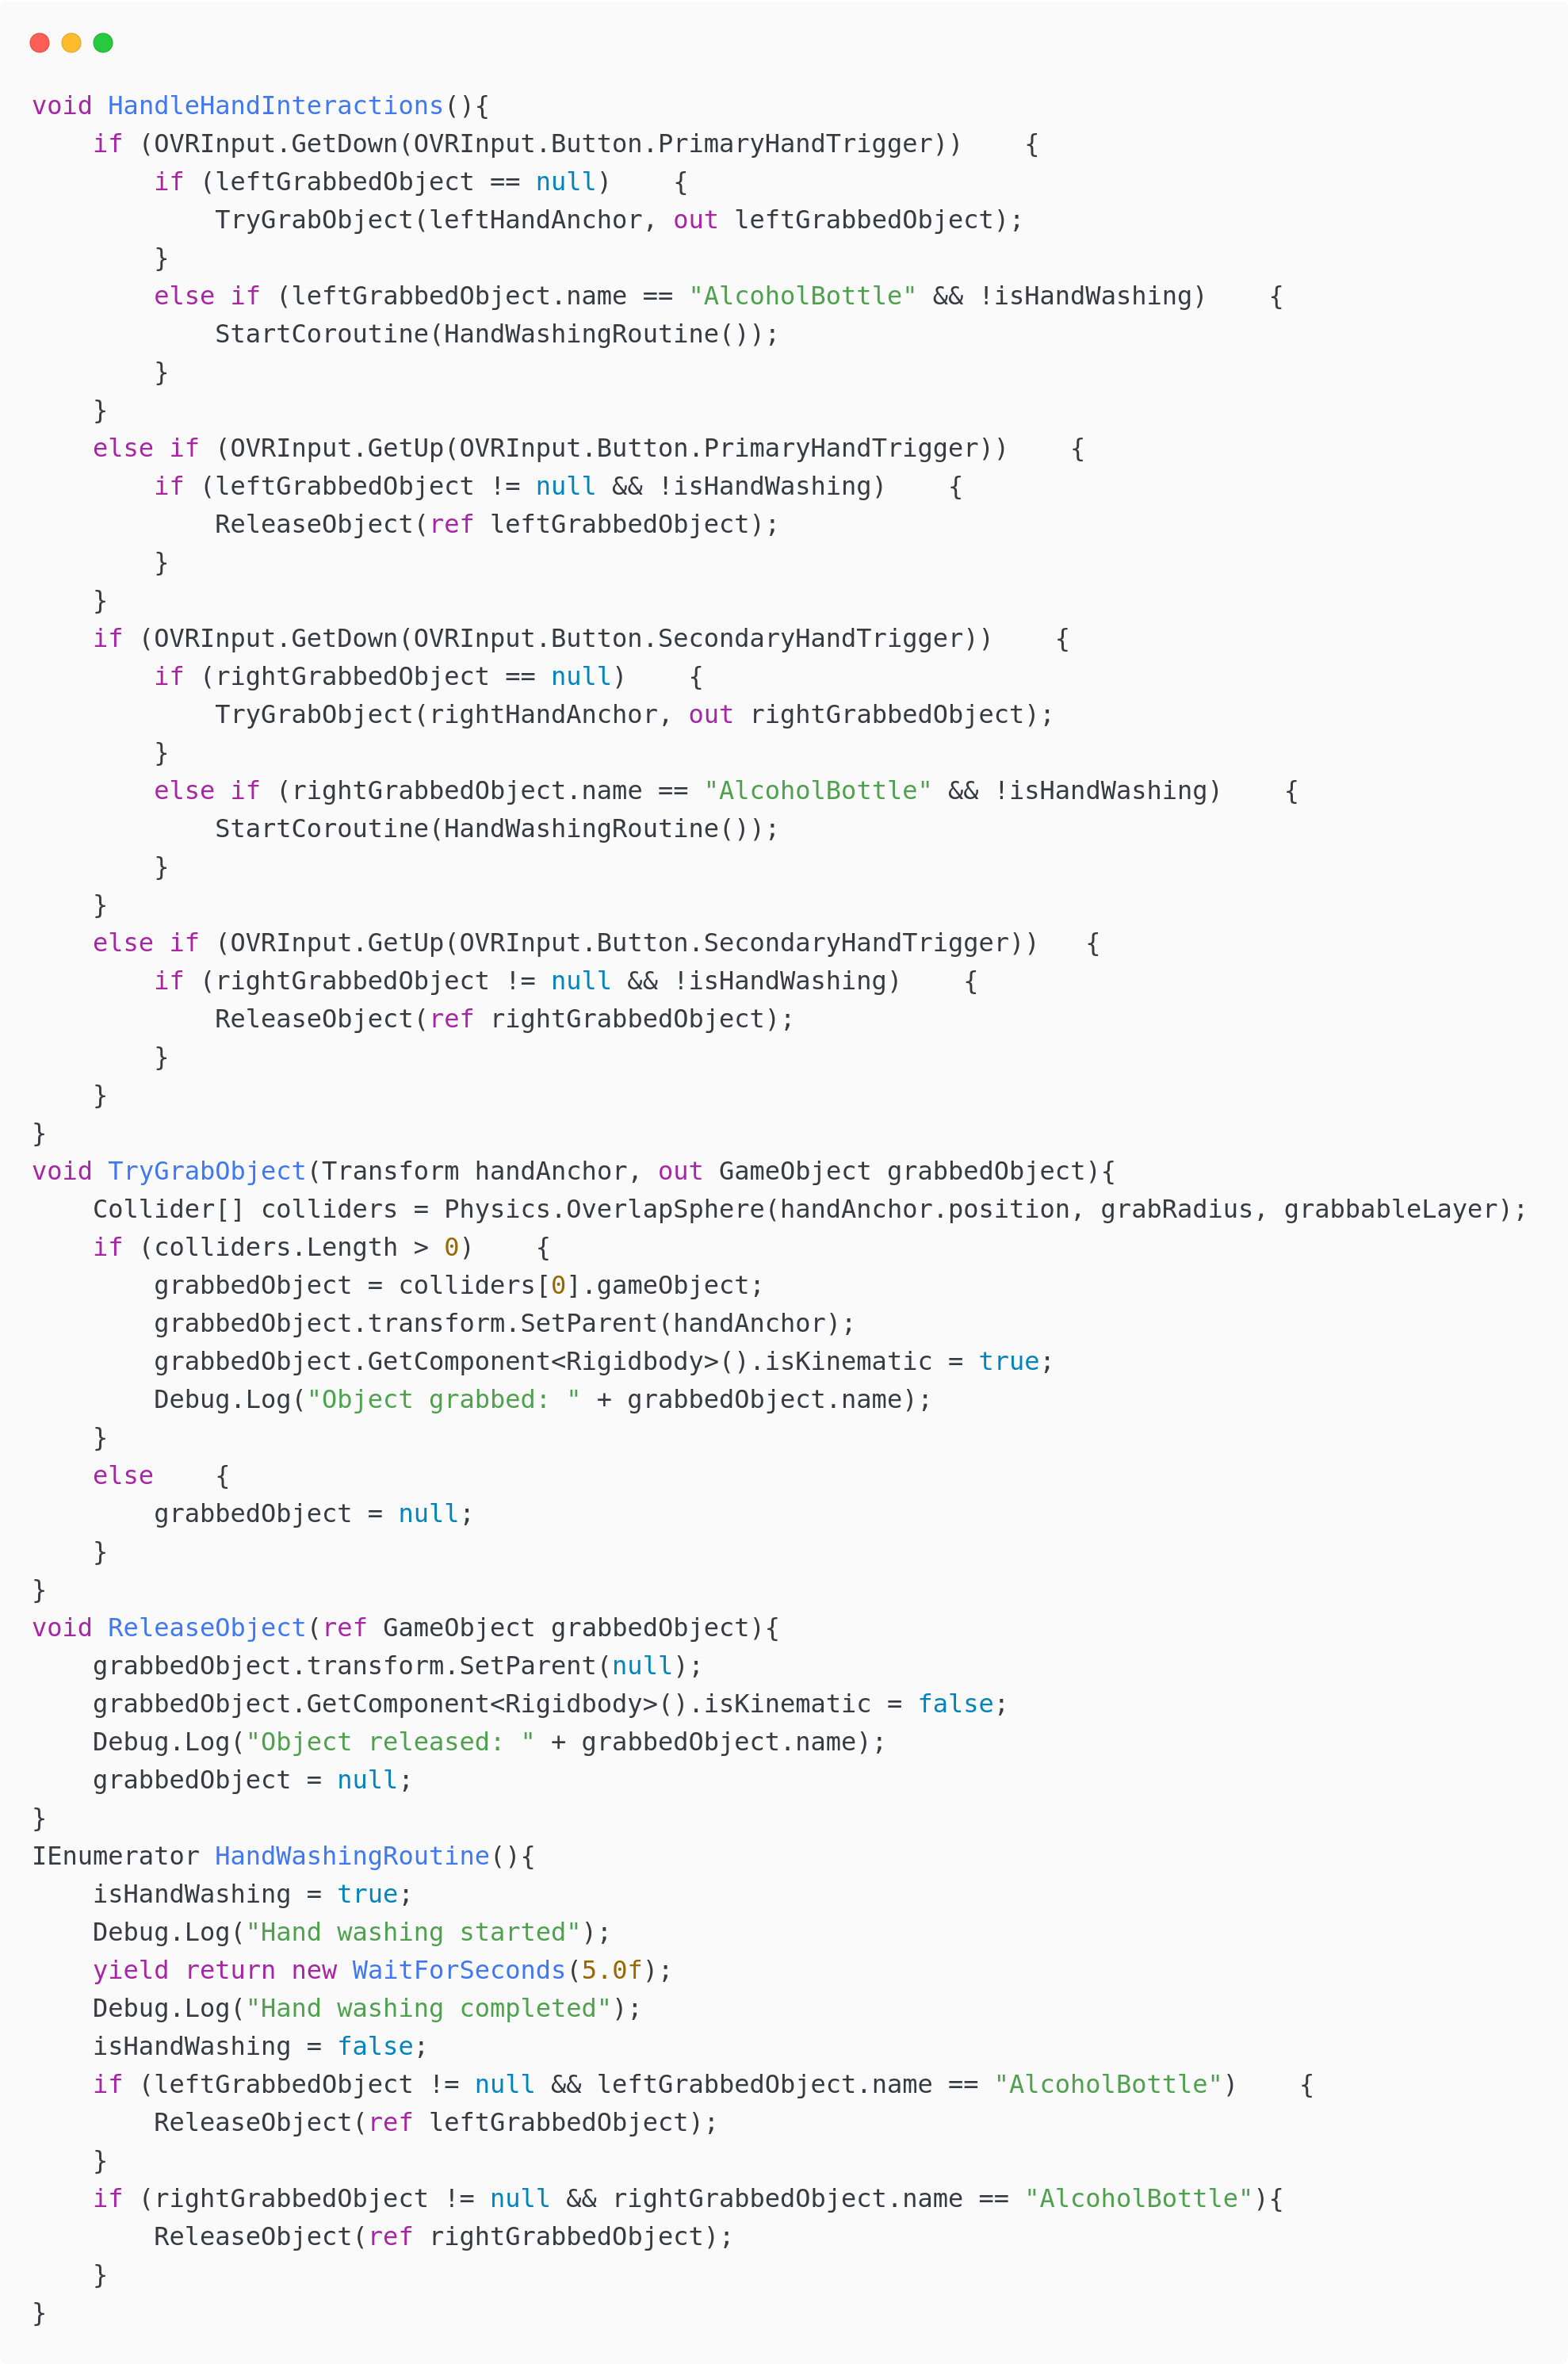
\includegraphics[width=1\textwidth, height=0.7\textheight]{Images/pore alcohol1.png}
	\caption{Pore Alcohol for Hands Washing}
	\label{fig:Grabbing-Tool}
\end{figure}
\newpage
\text{Code for Cleaning Injection Site Part of Body.}
\newline
\begin{figure}[h] 
	\centering
	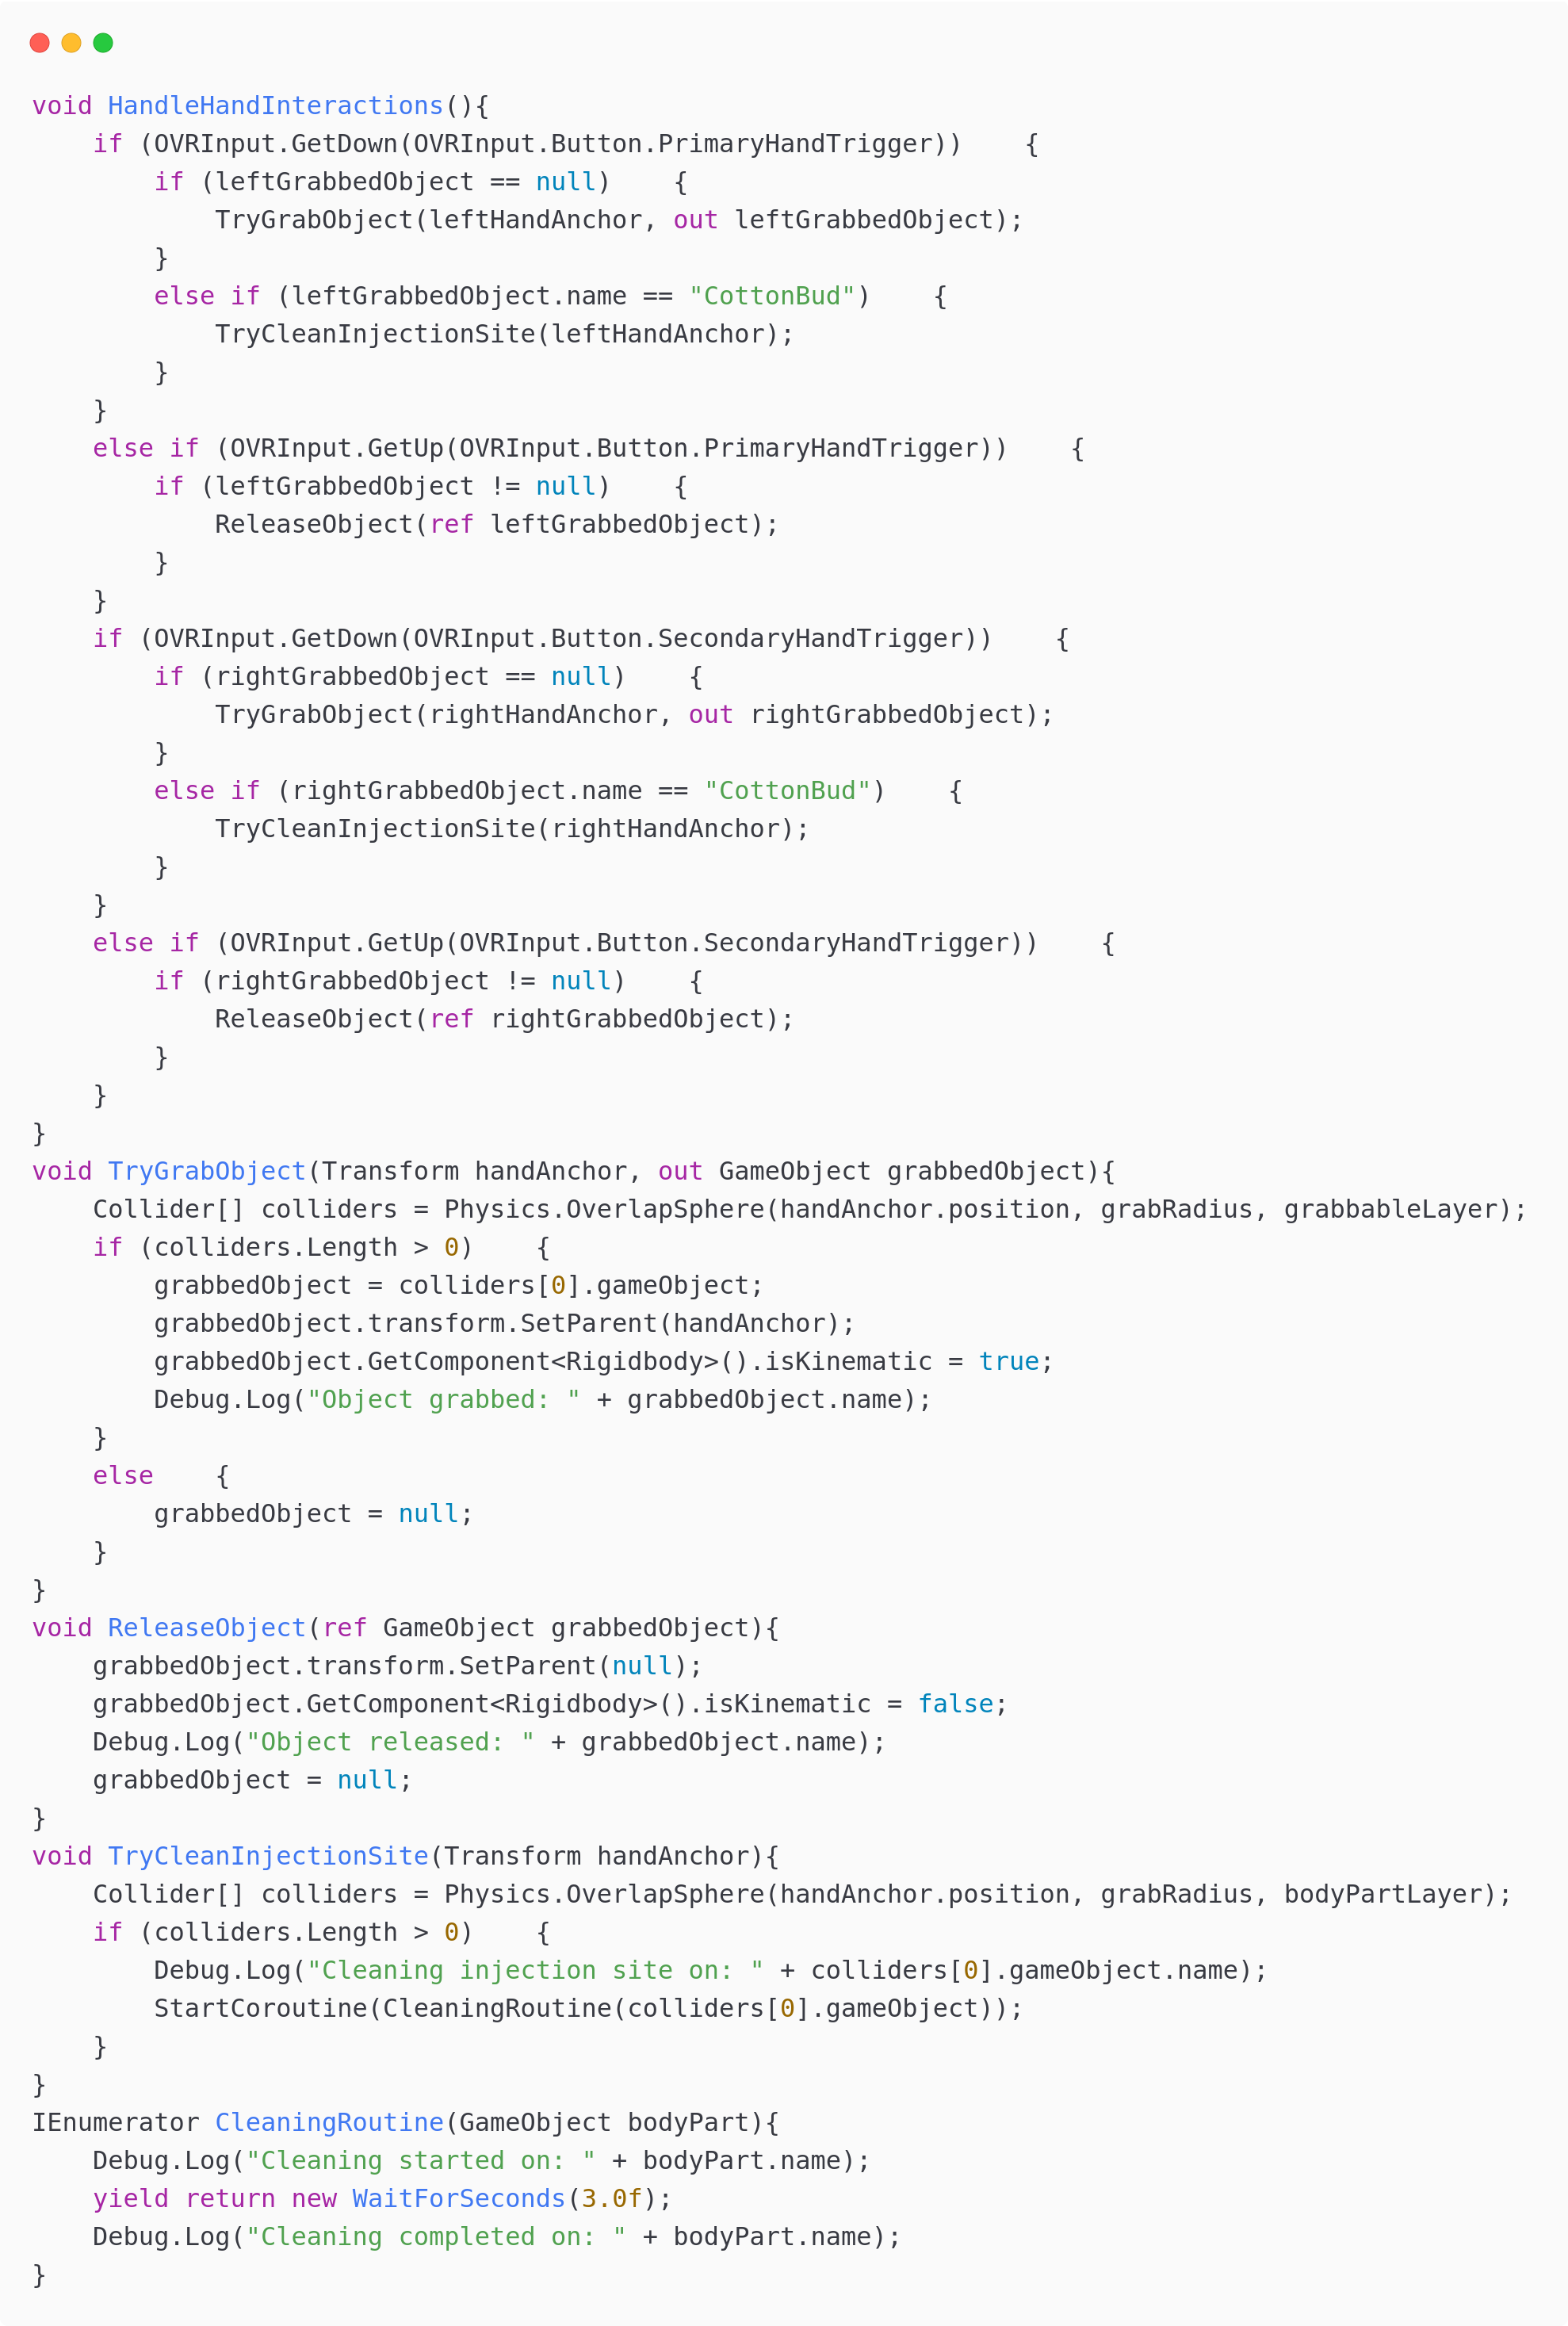
\includegraphics[width=1\textwidth, height=0.7\textheight]{Images/cleaning1.png}
	\caption{Cleaning Injection Site Part}
	\label{fig:Cleaning Injection Site Part}
\end{figure}
\newpage
	\text{ Code for Inject Syringe in Body.}
	\newline
\begin{figure}[h] 
	\centering
	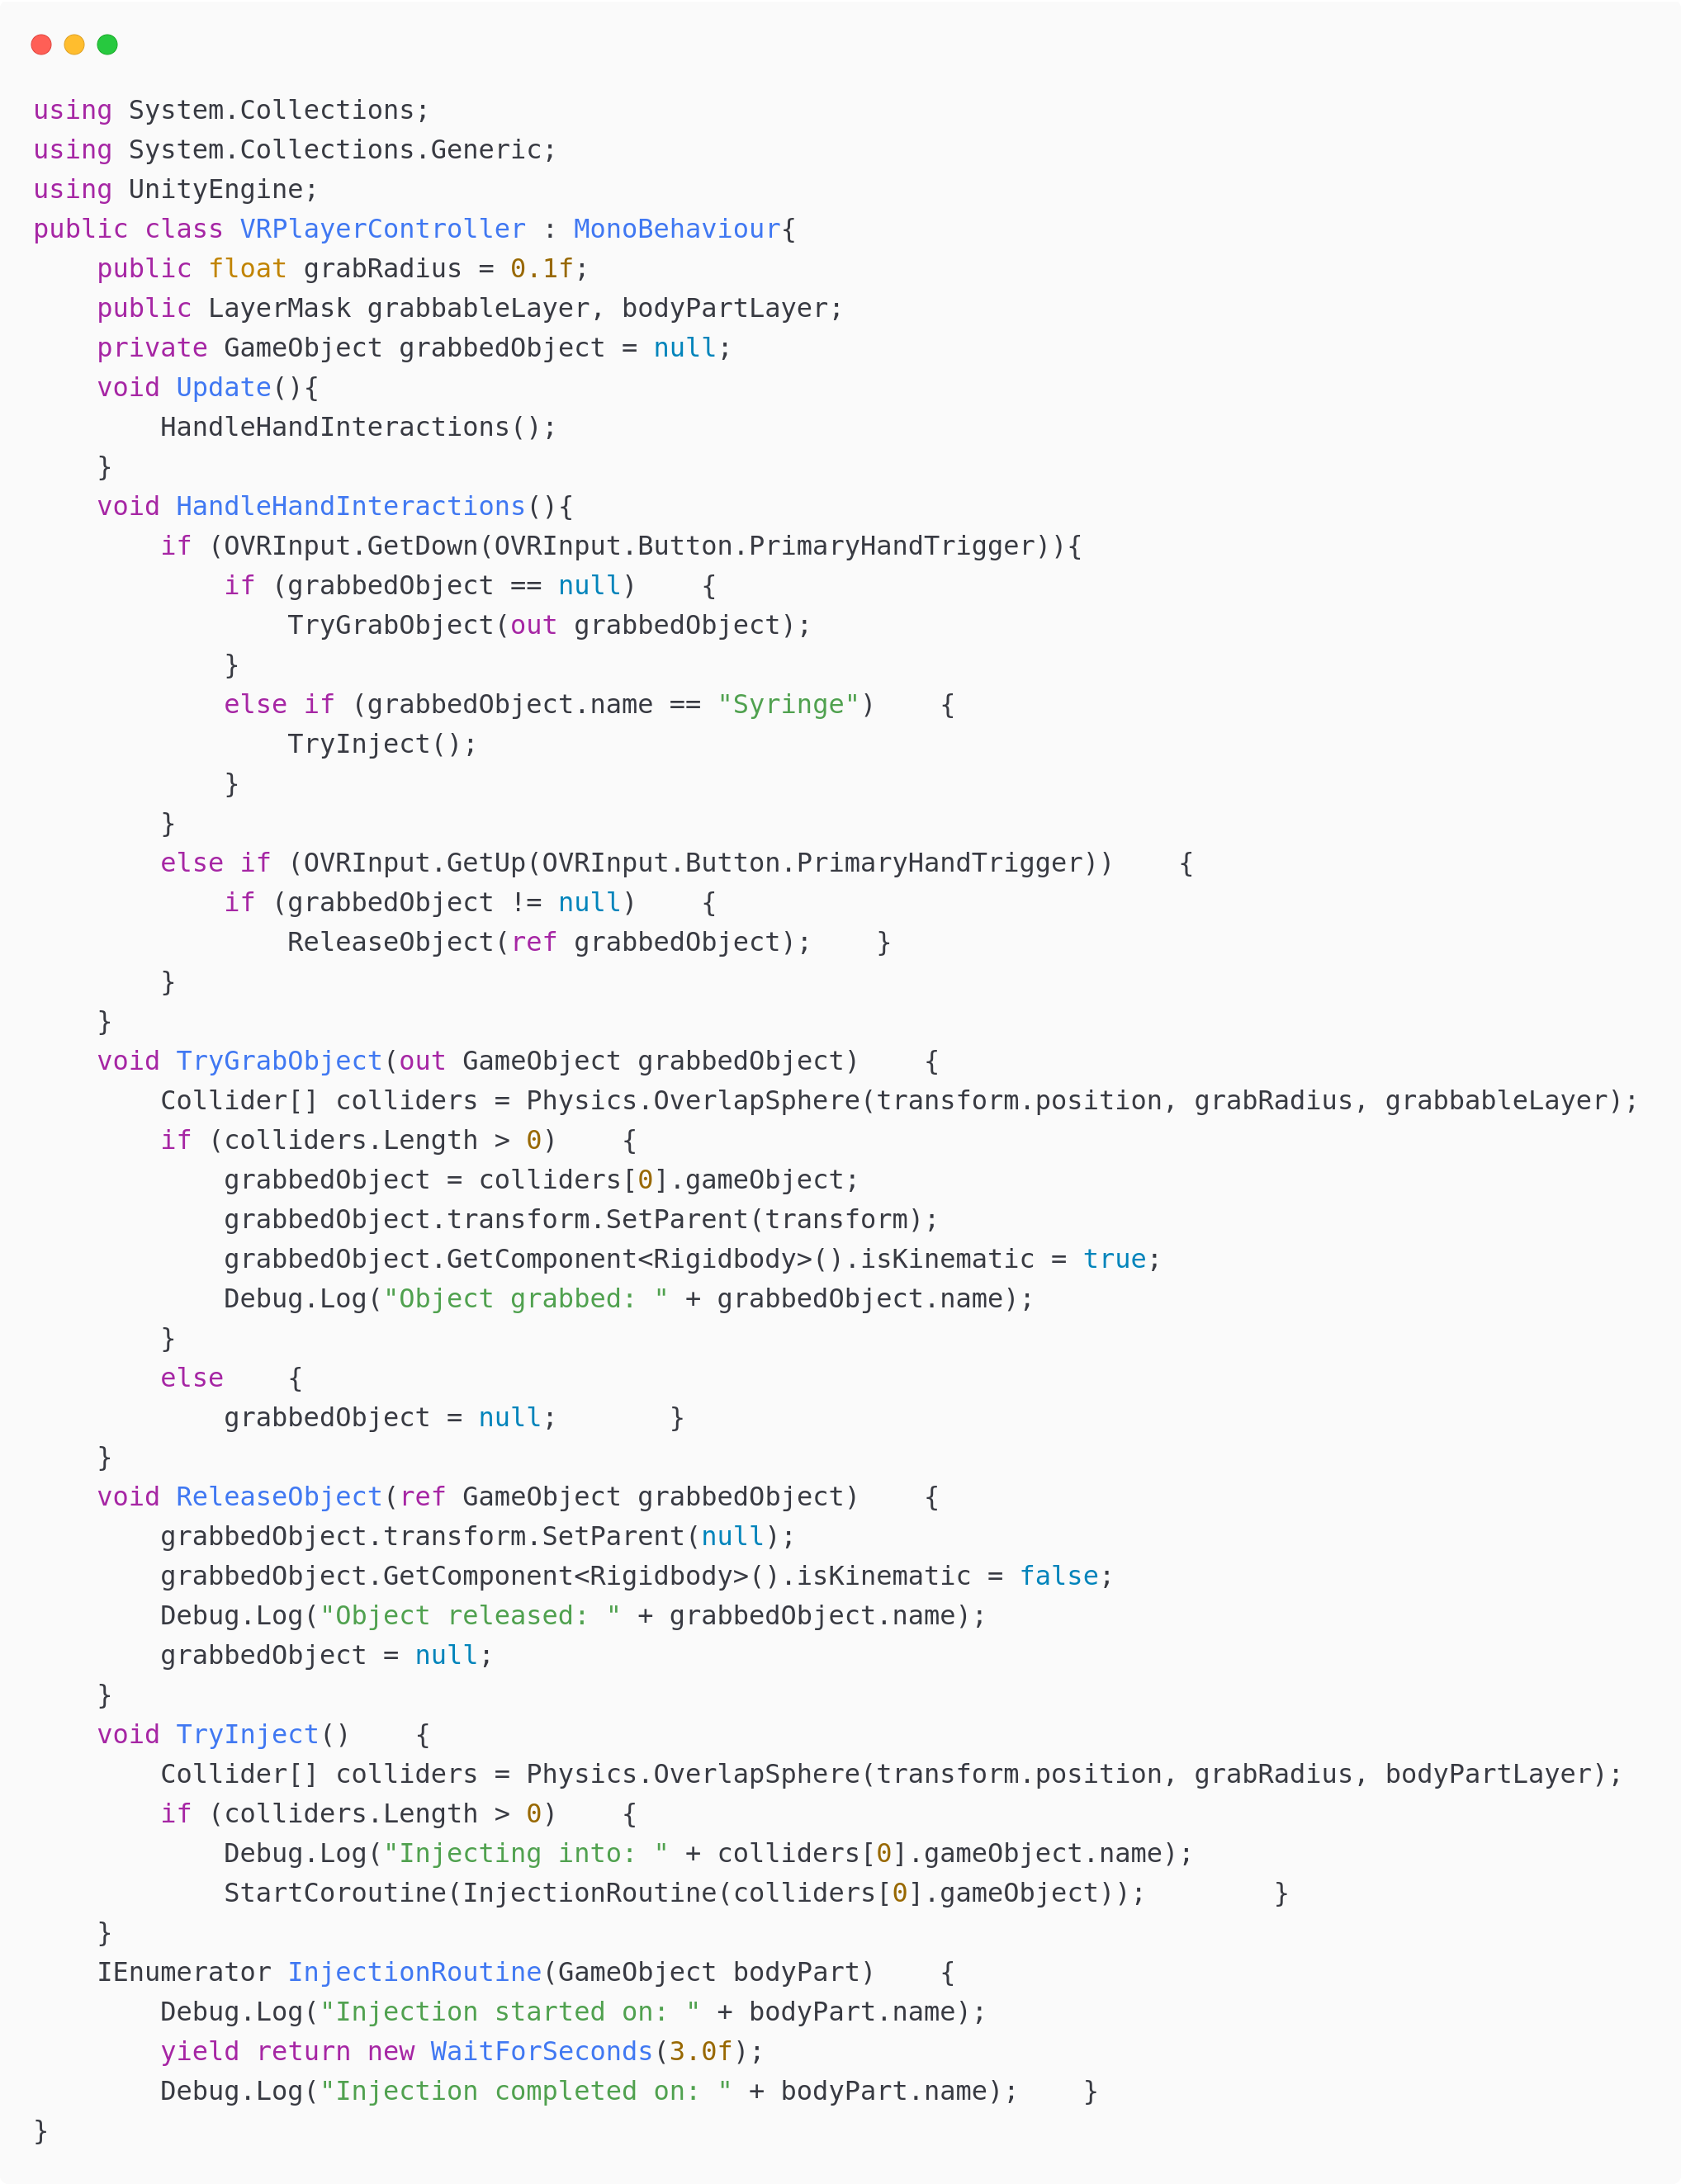
\includegraphics[width=1\textwidth, height=0.7\textheight]{Images/inject syringe.png}
	\caption{Inject Syringe in Body}
	\label{fig:Inject Syringe in Body}
\end{figure}
\newpage
\text{Code for Applying Cut and Bandage on Body.}
\newline
\begin{figure}[h] 
	\centering
	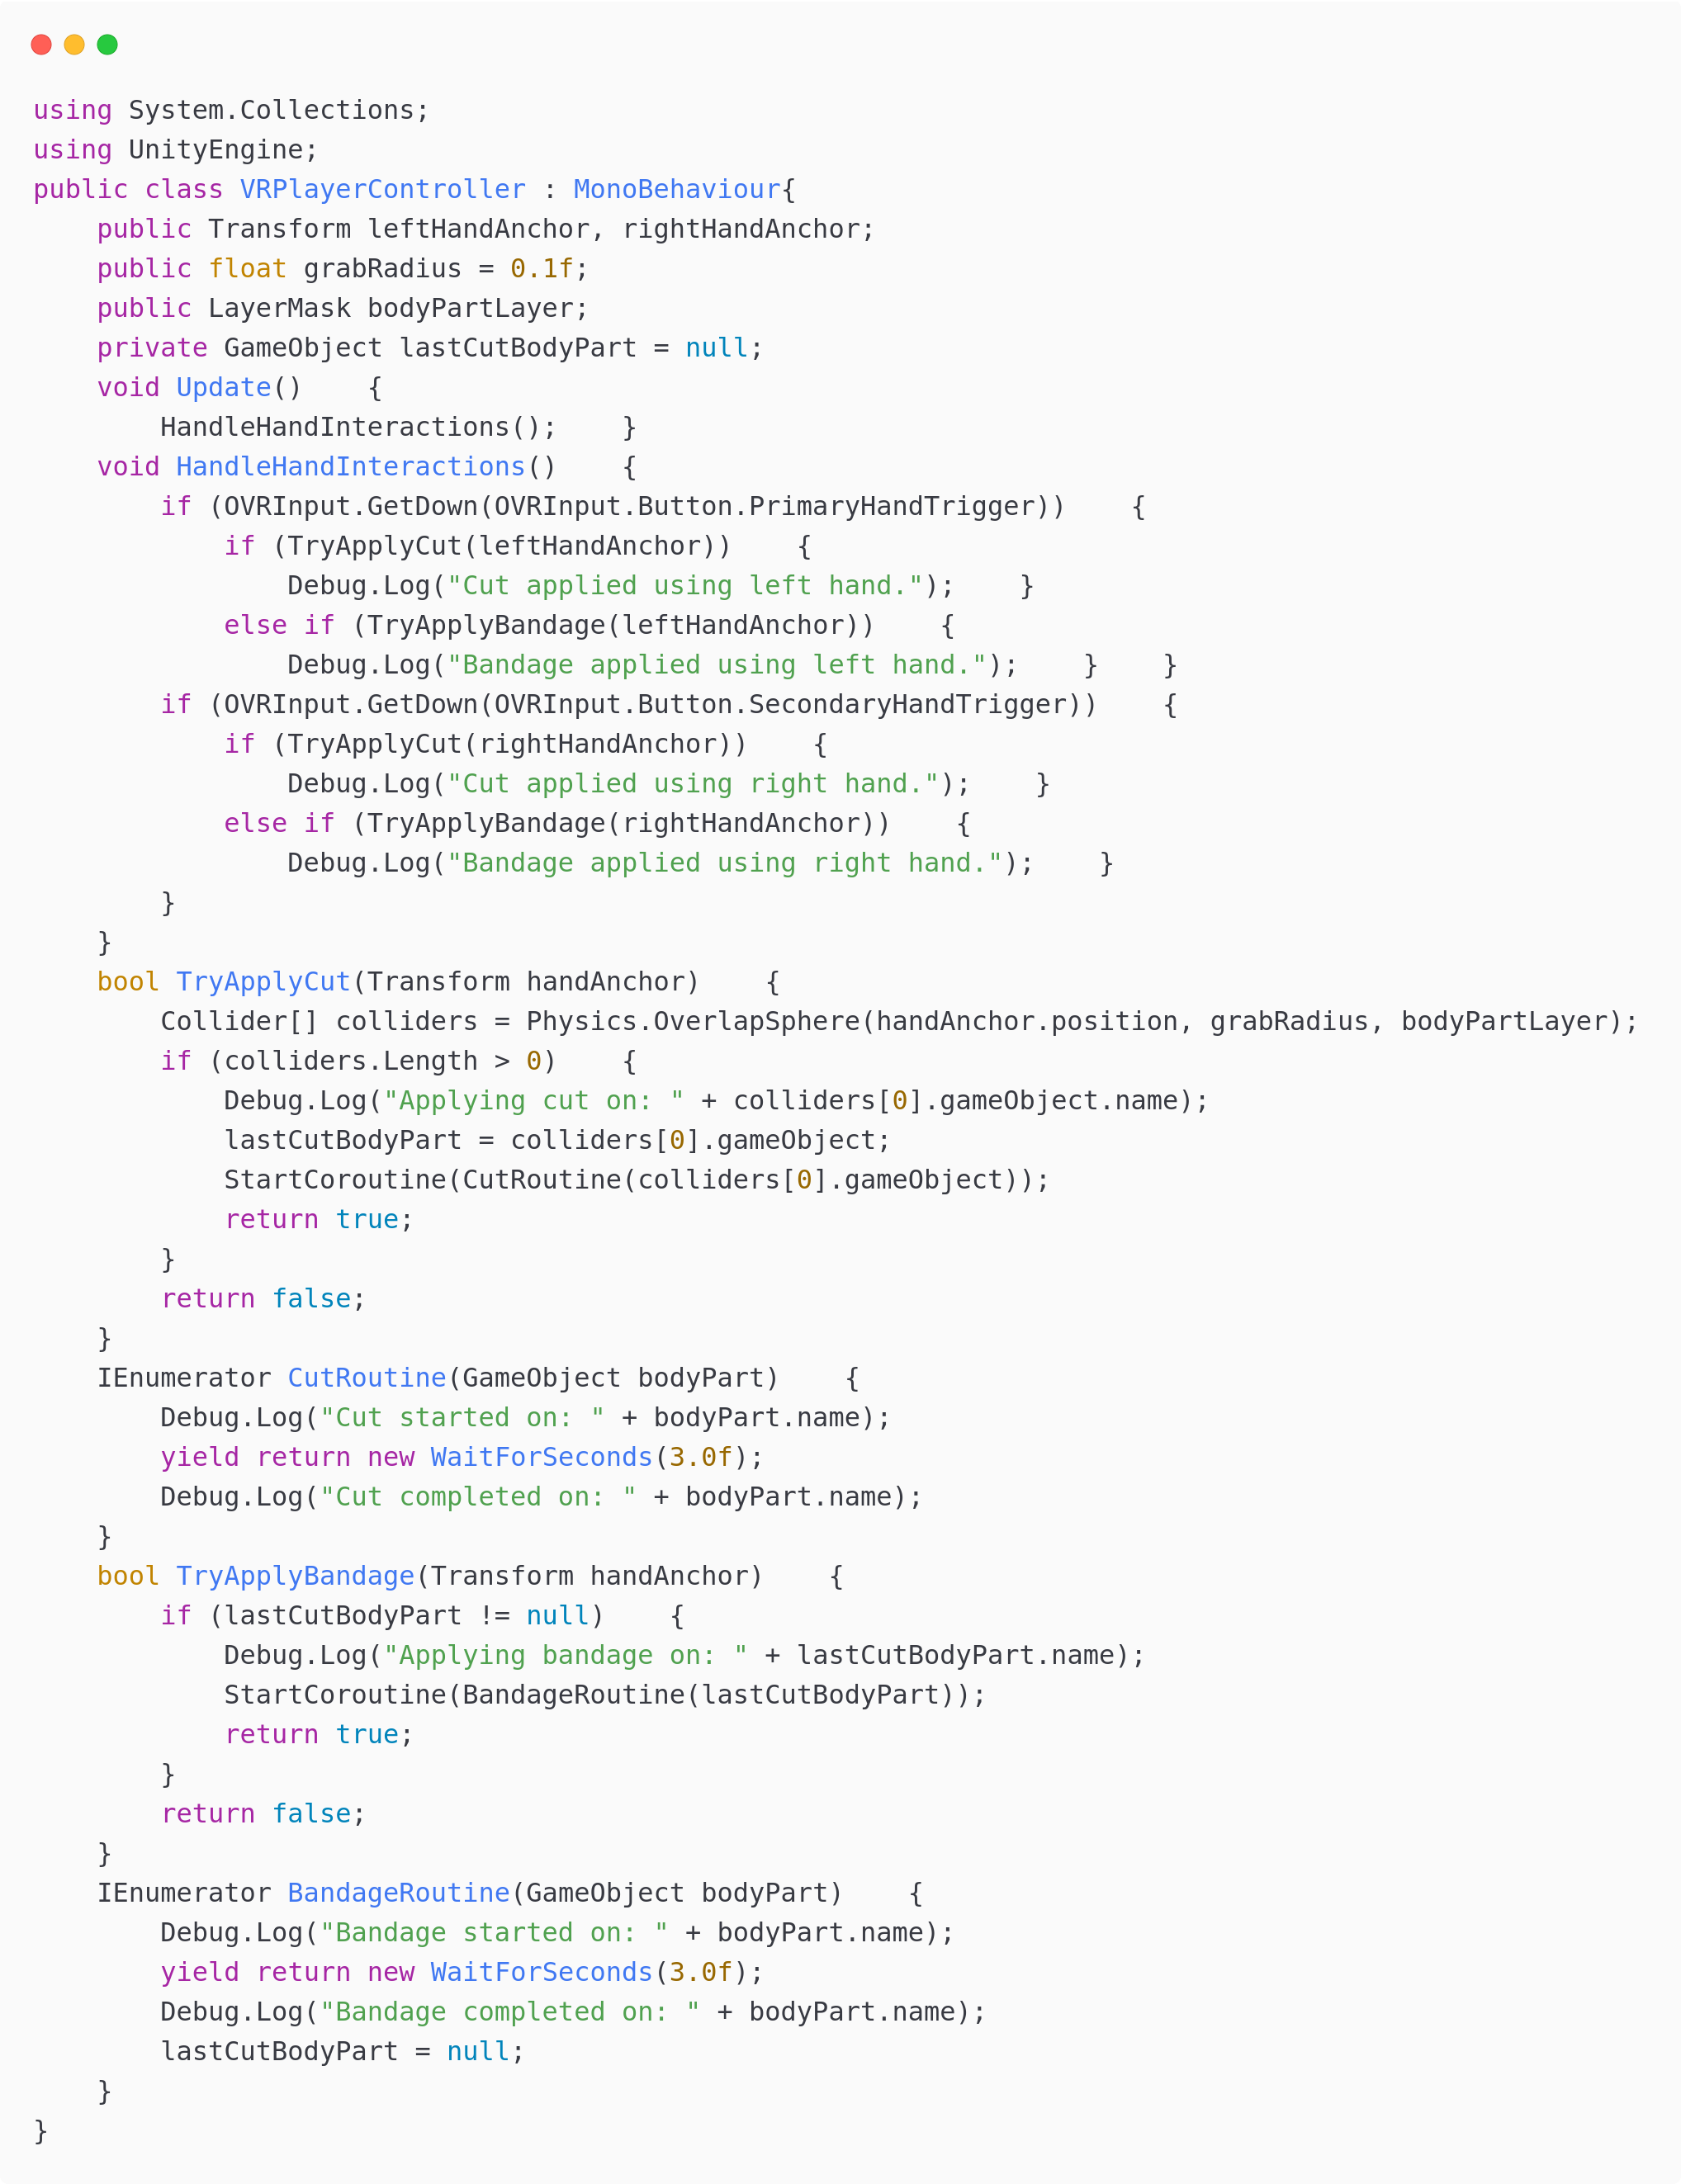
\includegraphics[width=1\textwidth, height=0.7\textheight]{Images/Applying Cut and Bandage on Body.png}
	\caption{Applying Cut and Bandage on Body}
	\label{fig:Applying Cut and Bandage on Body}
\end{figure}
\section{SVN or GitHub}
 Here is the GitHub link: \\
\href{https://github.com/Daudsarfraz/MetaMed}{https://github.com/Daudsarfraz/MetaMed}
	\chapter{Iteration 4}
\label{ch:iter4}
Meta-Med VR project's fourth iteration enhances user experience by integrating Keyboard and Meta Quest 2 functionalities, improving immersion, realism, and educational value for healthcare professionals.
\section{Introduction}
Meta-Med VR is a revolutionary approach that aims to enhance medical education by providing immersive virtual reality experiences for training and skill development.\\
\textbf{Integration Focus:}\\
This document focuses on the integration of Keyboard and Meta Quest 2 to enhance object interaction and movement within the Meta Med VR environment, aiming to improve user engagement and learning outcomes.
\section{Integration Process with Keyboard}
We evaluated several input devices based on factors such as compatibility, affordability, and ease of use. After careful consideration, we chose Keyboard for its versatility and familiarity to users.\\
\textbf{Compatibility Assessment:}\\
The MetaMed VR software underwent rigorous compatibility tests to ensure seamless integration, verifying hardware specifications and assessing software support for keyboard inputs.\\
\textbf{Software Configuration:}\\
Custom software configurations were created to enable recognition and response to keyboard inputs in the MetaMed VR environment, mapping keyboard keys to specific actions or functions.\\
\textbf{Testing and Calibration:}\\
The integration underwent rigorous testing to ensure smooth object interaction and movement, with calibration procedures implemented to optimize performance and reduce input latency.\\
\textbf{Enhancements and Features:}\\ 
Users can manipulate virtual objects using keyboard inputs, performing actions like grabbing, rotating, and moving objects within the VR space.\\
\textbf{Movement Controls:}\\
The keyboard integration offers users intuitive movement controls, including locomotion and teleportation options, facilitating seamless navigation through virtual environments.\\
\textbf{User Experience Improvements:}\\
The integration improves immersion and realism in the MetaMed VR environment, enhancing engagement and effectiveness in training scenarios.
\section{Integration Process with Meta Quest 2}
\textbf{Selection of Meta Quest 2:}\\
We selected Meta Quest 2 due to its advanced features and user-friendly interface after evaluating various input devices for compatibility, affordability, and tracking capabilities.\\
\textbf{Compatibility Assessment:}\\
The integration of MetaMed VR software was ensured through rigorous compatibility tests, verifying hardware specifications and assessing software support for Meta Quest 2 inputs.\\
\textbf{Software Configuration:}\\
Custom software configurations were created to enable recognition and response to Meta Quest 2 inputs within the MetaMed VR environment, including integrating Meta Quest 2.
\section{Testing and Calibration}
\textbf{Testing Procedures:}\\
The integration underwent rigorous testing to ensure smooth object interaction and movement, with calibration procedures implemented to optimize tracking accuracy and minimize latency.
\section{Enhancements and Features}
Meta Quest 2 enables users to interact with virtual objects through gestures like grabbing, rotating, and moving within the VR space. Meta Quest 2's integration offers users intuitive movement controls, including locomotion and teleportation options, facilitating seamless navigation through virtual environments.\\
The integration improves immersion and realism in the MetaMed VR environment, enhancing engagement and effectiveness in training scenarios.
\section{Challenges and Solutions}
The integration process faced technical issues like input latency and mapping conflicts.\\
The challenges were resolved through software updates, configuration adjustments, and calibration procedures to guarantee a seamless user experience.
\section{Future Directions}
Future improvements include improving input mappings, enhancing keyboard shortcut support, improving gesture recognition algorithms, and introducing advanced hand tracking features.
\section{Conclusion}
The integration of Keyboard and Meta Quest 2 with $MetaMed$ VR is a significant advancement in medical education through immersive virtual reality experiences. $MetaMed$ VR enhances healthcare professional training and patient care outcomes by improving object interaction and movement controls.
	\chapter{Implementation Details}
\label{ch:implementation}
{Here are some implementation details of project. What we can do in project.}
\section{Introduction}
This essay explores the use of Meta Quest 2 and the various Libraries to create a comprehensive virtual training environment for medical practitioners, detailing the process from user authentication to performing procedures in a virtual hospital setting, showcasing Virtual Reality's potential in medical education.
\section{User Authentication and Environment Access}
The training uses Meta Quest 2, a high-resolution virtual environment, with keyboard navigation. Authentication involves signing up through the meta-verse or Meta-Mask, ensuring security. Correct credentials grant access, while incorrect ones prompt a new sign-up, ensuring integrity and integrity.
\section{Navigation to the Virtual Hospital Environment}
Upon successful authentication, users are transported to a meticulously crafted virtual hospital environment, allowing navigation through various areas such as wards, operation theaters, laboratories, and administrative sections, enhancing the training experience.
\section{Scenario Selection and Patient Interaction}
Users visit the reception area to select an interactive training scenario from various patient cases, covering various medical conditions. They then practice diagnostic and treatment skills in a controlled, risk-free environment by observing detailed patient histories, symptoms, and physical examinations in the designated patient.
\section{Laboratory Interaction and Tool Acquisition}
Users choose a patient scenario and visit a virtual laboratory to gather tools and medications. The VR environment simulates a fully-equipped lab, allowing users to practice selecting and handling medical instruments. Some open-source frameworks enhance realism and training effectiveness.
\section{Performing Medical Procedures}
Users use VR to perform medical procedures, providing step-by-step guidance and real-time feedback. The immersive nature allows users to experience procedural nuances, such as injections, wound suturing, and diagnostic equipment usage.
\section{Exit from the Virtual Environment}
The user exits the virtual environment after completing the training scenario, allowing easy transition back to the real world, and the training sessions can be repeated for skill development and refinement.

 
	\chapter{User Manual}
\label{ch:manual}
This chapter will have the user manual. These UI/UX elements are crafted to be responsive and visually appealing, ensuring a seamless and enjoyable experience for users as they practice medical procedures and scenarios.
\section{Choose Scenario}
Users start by selecting a scenario corresponding to a patient's medical issue from a menu of various conditions or scenarios.
\begin{figure}[h]
    \centering
    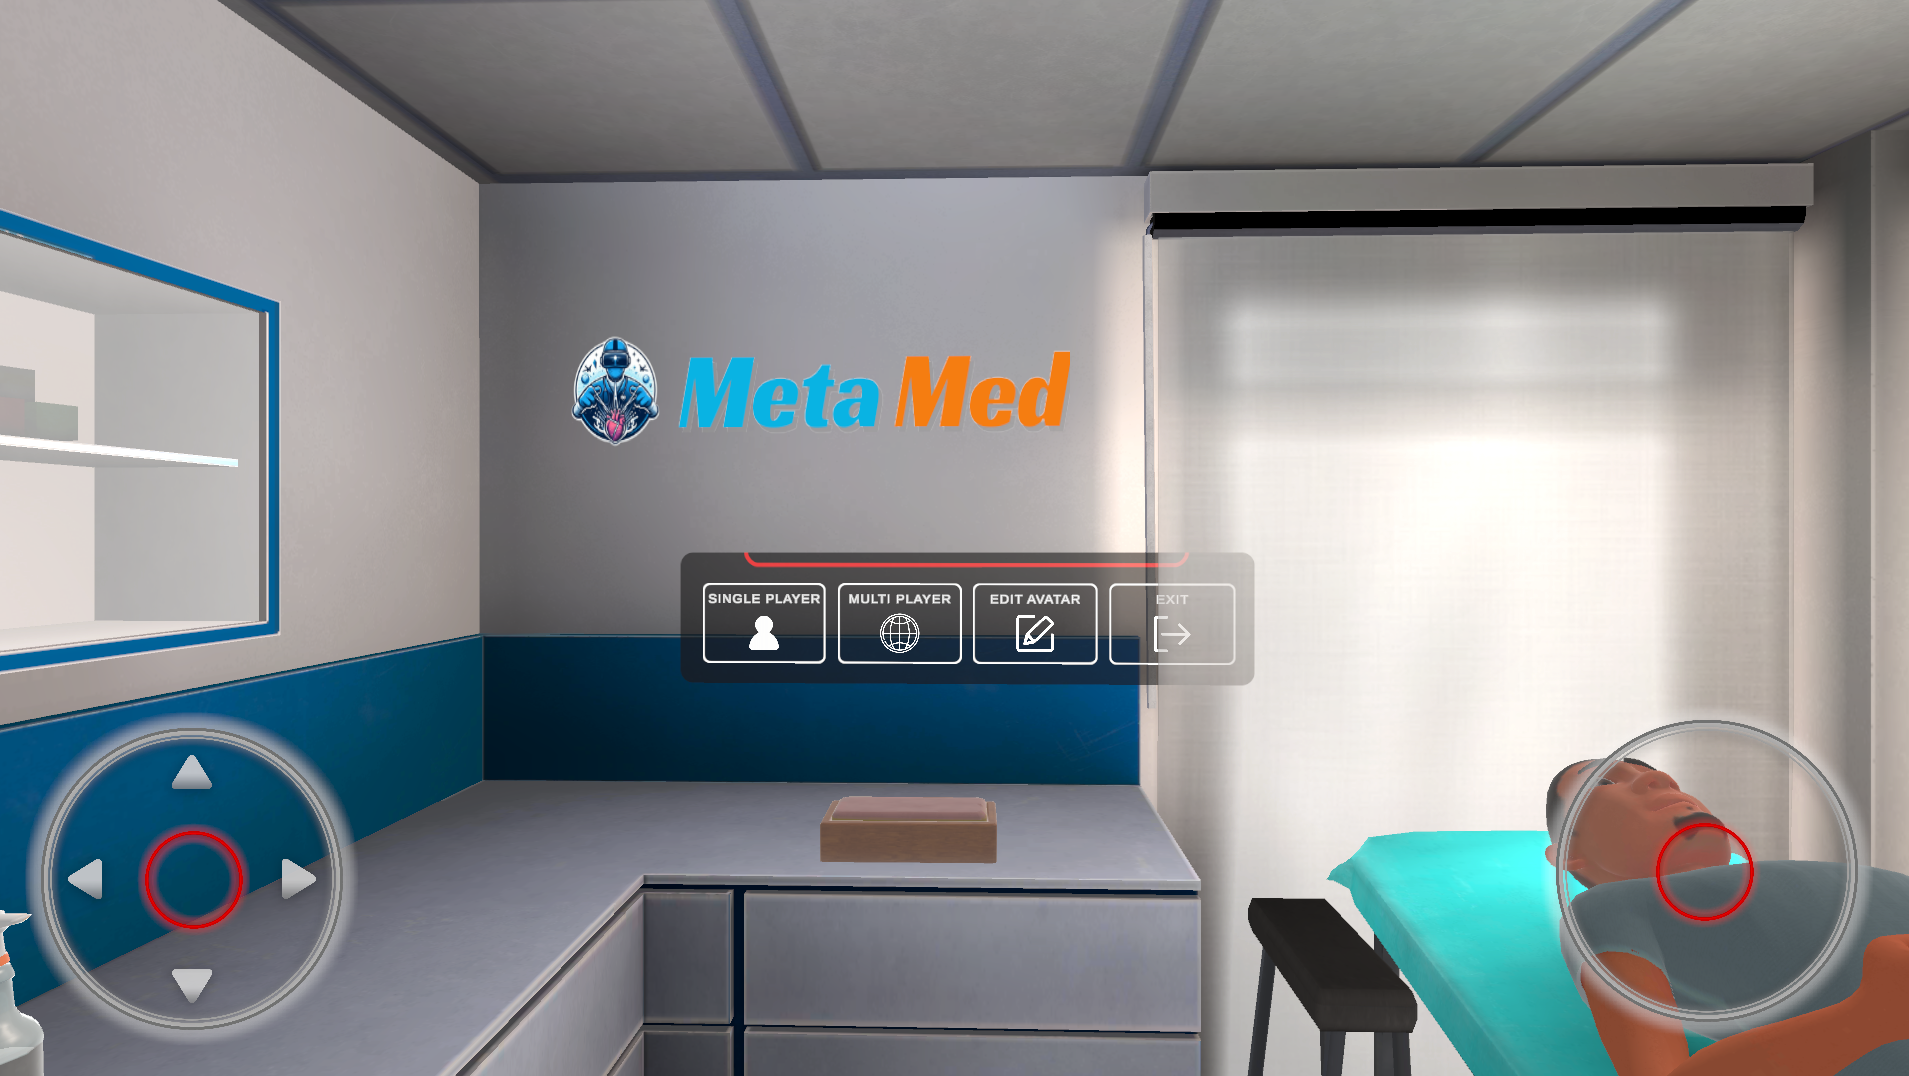
\includegraphics[width=0.7\textwidth, height=0.3\textheight]{Images/User Manual.png}
    \caption{User Manual}
    \label{fig:User Manual}
\end{figure}

\section{Start Session}
When session start other user can interact with you.
\begin{figure}[h]
	\centering
	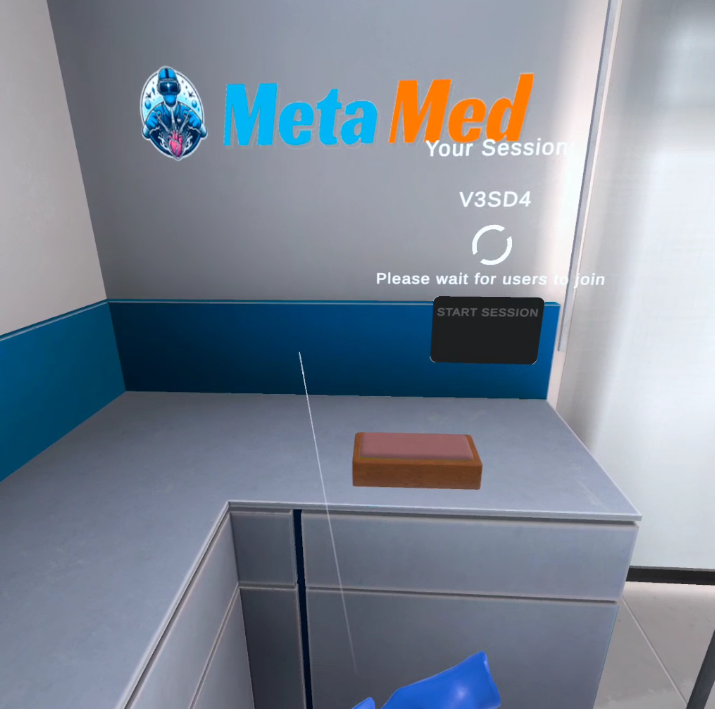
\includegraphics[width=0.7\textwidth, height=0.3\textheight]{Images/start session.png}
	\caption{Start Session}
	\label{fig:Start Session}
\end{figure}

\section{Choose Scenario}
Here can choose scenario like operation of leg, arm, foot etc.
\begin{figure}[h]
	\centering
	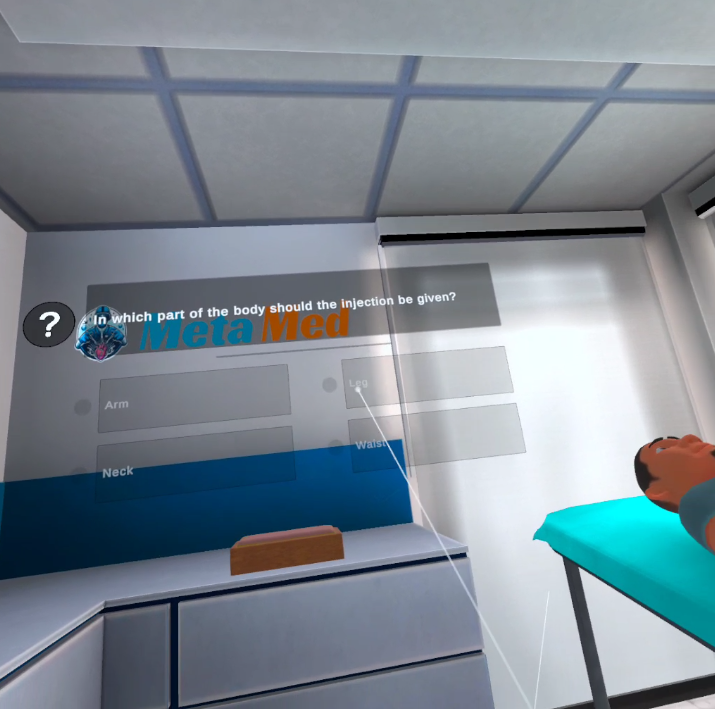
\includegraphics[width=0.7\textwidth, height=0.3\textheight]{Images/select body part.png}
	\caption{Choose Scenario}
	\label{fig:ChooseScenario}
\end{figure}
	\chapter{Conclusions and Future Work}
In this chapter we have defined which features can be implement in Future.
\section{Conclusion:}
Our $metaverse$ project's basic capabilities, such as injection procedures, patient records, and medication records, have been effectively built throughout its first development. The foundation for a strong, engaging, and extremely useful virtual healthcare environment is laid by these fundamental instruments. But in order for this $metaverse$ healthcare system to reach its full potential, a few things need to be improved and developed further.
\section{Future Work:}
Future research will focus on advanced clinical simulations, real-time feedback, and virtual diagnostic tools like blood tests, CT, and MRI scans. Emergency training scenarios will incorporate time-sensitive decision-making and multi-user cooperation. AI-driven virtual consultations, comprehensive patient histories, and secure communication will enhance patient interaction. Therapeutic environments will offer interactive modules for education, rehabilitation, and mental health therapy. Key priorities include interoperability with healthcare systems, IoT device integration, and blockchain for secure records. Educational resources will expand through interactive modules, virtual dissection labs, and online CME in the metaverse. User experience will be improved with a user-friendly interface, multilingual support, cultural adaptations, and accessibility features.
	
	%\appendix
	% \chapter{Appendix I title}
 
 text here

	
	\bibliographystyle{plain}
	\bibliography{bib} 
	\addcontentsline{toc}{chapter}{References} 
	
\end{document}